\documentclass{article}

% if you need to pass options to natbib, use, e.g.:
%     \PassOptionsToPackage{numbers, compress}{natbib}
% before loading neurips_2026

% The authors should use one of these tracks.
% Before accepting by the NeurIPS conference, select one of the options below.
% 0. "default" for submission
\usepackage[preprint]{neurips_2026}
% the "default" option is equal to the "main" option, which is used for the Main Track with double-blind reviewing.
% 1. "main" option is used for the Main Track
%  \usepackage[main]{neurips_2026}
% 2. "position" option is used for the Position Paper Track
%  \usepackage[position]{neurips_2026}
% 3. "eandd" option is used for the Evaluations & Datasets Track
 % \usepackage[eandd]{neurips_2026}
 % if you need to opt-in for a single-blind submission in the E&D track:
 %\usepackage[eandd, nonanonymous]{neurips_2026}
% 4. "creativeai" option is used for the Creative AI Track
%  \usepackage[creativeai]{neurips_2026}
% 5. "sglblindworkshop" option is used for the Workshop with single-blind reviewing
 % \usepackage[sglblindworkshop]{neurips_2026}
% 6. "dblblindworkshop" option is used for the Workshop with double-blind reviewing
%  \usepackage[dblblindworkshop]{neurips_2026}

% After being accepted, the authors should add "final" behind the track to compile a camera-ready version.
% 1. Main Track
 % \usepackage[main, final]{neurips_2026}
% 2. Position Paper Track
%  \usepackage[position, final]{neurips_2026}
% 3. Evaluations & Datasets Track
 % \usepackage[eandd, final]{neurips_2026}
% 4. Creative AI Track
%  \usepackage[creativeai, final]{neurips_2026}
% 5. Workshop with single-blind reviewing
%  \usepackage[sglblindworkshop, final]{neurips_2026}
% 6. Workshop with double-blind reviewing
%  \usepackage[dblblindworkshop, final]{neurips_2026}
% Note. For the workshop paper template, both \title{} and \workshoptitle{} are required, with the former indicating the paper title shown in the title and the latter indicating the workshop title displayed in the footnote.
% For workshops (5., 6.), the authors should add the name of the workshop, "\workshoptitle" command is used to set the workshop title.
% \workshoptitle{WORKSHOP TITLE}

% "preprint" option is used for arXiv or other preprint submissions
 % \usepackage[preprint]{neurips_2026}

% to avoid loading the natbib package, add option nonatbib:
%    \usepackage[nonatbib]{neurips_2026}

\usepackage[utf8]{inputenc} % allow utf-8 input
\usepackage[T1]{fontenc}    % use 8-bit T1 fonts
\usepackage{hyperref}       % hyperlinks
\usepackage{url}            % simple URL typesetting
\usepackage{booktabs}       % professional-quality tables
\usepackage{amsfonts}       % blackboard math symbols
\usepackage{nicefrac}       % compact symbols for 1/2, etc.
\usepackage{microtype}      % microtypography
\usepackage{xcolor}         % colors
\usepackage{graphicx}
\usepackage{amsmath}
\usepackage{multirow}
\usepackage{placeins}
\graphicspath{{figures/}}

% Note. For the workshop paper template, both \title{} and \workshoptitle{} are required, with the former indicating the paper title shown in the title and the latter indicating the workshop title displayed in the footnote. 
\title{A Hybrid Clustering and Classification Framework for Predicting Student Dropout and Academic Success}


% The \author macro works with any number of authors. There are two commands
% used to separate the names and addresses of multiple authors: \And and \AND.
%
% Using \And between authors leaves it to LaTeX to determine where to break the
% lines. Using \AND forces a line break at that point. So, if LaTeX puts 3 of 4
% authors names on the first line, and the last on the second line, try using
% \AND instead of \And before the third author name.


\author{%
  Zachary Adam\\
  Department of Computer Science\\
  Rutgers University\\
  New Brunswick - Piscataway, NJ \\
  \texttt{zachary.adam@rutgers.edu} \\
}


\begin{document}


\maketitle


\begin{abstract}
Student retention is a major challenge in higher education because academic dropout can negatively affect students, institutions, and broader educational outcomes. This project studies whether combining unsupervised student segmentation with supervised machine learning can improve the prediction and interpretation of academic outcomes. Using a higher-education student retention dataset, I formulate the task as a three-class classification problem: predicting whether a student will drop out, remain enrolled, or graduate. The proposed workflow applies structured preprocessing, including binary mapping, one-hot encoding of categorical variables, and scaling of numerical variables. I then compare baseline supervised models against cluster-augmented models that incorporate K-Means student segments as additional features. The best overall model was a baseline Random Forest, which achieved 0.7605 accuracy and 0.8902 macro ROC-AUC. Logistic Regression achieved the highest macro F1-score of 0.6852, indicating stronger balance across the imbalanced classes. K-Means clustering did not consistently improve predictive accuracy when added as a feature, but it revealed interpretable student-risk profiles, including a high-risk cluster with 82.0\% dropout. These results suggest that supervised models capture most predictive structure directly from academic and enrollment features, while clustering remains useful as an interpretability tool for identifying distinct student groups.
\end{abstract}

\section{Introduction}

Student dropout is an important problem in higher education because it can affect student well-being, institutional planning, graduation rates, and the efficient use of academic support resources. Universities often collect large amounts of structured student data, including demographic information, enrollment records, socioeconomic variables, and academic performance indicators. When used carefully, these data can support early warning systems that identify students who may need additional advising, tutoring, financial support, or other interventions.

The goal of this project is to predict student academic outcomes using machine learning. Specifically, I study a three-class classification task in which each student is labeled as \textit{Dropout}, \textit{Enrolled}, or \textit{Graduate}. This setting is more realistic than a binary pass/fail problem because students may remain enrolled without graduating by the normal course duration. However, the multiclass formulation also introduces additional difficulty because the target classes are imbalanced: in this dataset, the \textit{Graduate} class is the largest class, while \textit{Enrolled} is substantially smaller.

This project is motivated by two connected questions. First, how accurately can standard supervised learning models predict student academic outcomes from tabular institutional data? Second, can unsupervised clustering improve either the predictive performance or interpretability of these models? To address these questions, I compare Logistic Regression, Random Forest, and Extra Trees classifiers under two pipelines: a baseline supervised pipeline and a cluster-augmented pipeline. In the cluster-augmented setting, K-Means is first used to segment students based on preprocessed features, and the resulting cluster labels are one-hot encoded and appended to the supervised feature matrix.

The main contribution of this project is not a new algorithm, but a complete and reproducible data science workflow for student retention prediction. The workflow includes data preprocessing, unsupervised segmentation, supervised classification, multiclass evaluation, feature importance analysis, and interpretation of student clusters. The complete code repository for reproducing the experiments is available at:
\href{https://github.com/zackadam0/CS439-student-retention-project}{github.com/zackadam0/CS439-student-retention-project}.

The results show that a baseline Random Forest achieved the strongest overall predictive performance, with 0.7605 accuracy and 0.8902 macro ROC-AUC. Logistic Regression produced the highest macro F1-score, indicating a better balance across classes. Adding cluster labels did not consistently improve performance, but the K-Means clusters provided meaningful interpretability. In particular, one cluster represented a high-risk student group with very low semester completion metrics and an 82.0\% dropout rate.

\section{Related Work}

\subsection{Educational data mining and dropout prediction}

Educational data mining applies statistical and machine learning methods to educational data in order to understand student behavior, predict outcomes, and support decision-making. Student dropout prediction is one of the most common applications of educational data mining because early identification of at-risk students can help institutions intervene before students permanently leave their programs.

Prior work has studied dropout prediction using administrative data, academic records, learning management system logs, and demographic variables. These studies commonly frame dropout prediction as a supervised learning problem in which models learn to classify students based on historical examples. Del Bonifro et al. developed a machine learning tool for first-year undergraduate dropout prediction, showing that data-driven approaches can support early identification of students at risk \citep{delbonifro2020dropout}. Prenkaj et al. surveyed machine learning approaches for student dropout prediction in online courses and emphasized that dropout prediction is a major task in learning analytics and educational data mining \citep{prenkaj2020survey}. More recent work has continued to study student dropout prediction using institutional and learning behavior data, often comparing traditional classifiers with more complex models \citep{goren2024early}.

The dataset used in this project was introduced by Realinho et al. for predicting student dropout and academic success in higher education \citep{realinho2022predicting}. The original dataset was designed to support early identification of students at risk of dropout or academic failure. Each instance represents a student, and the features include information about academic path, demographics, socioeconomic context, and first- and second-semester academic performance. This makes the dataset appropriate for studying both predictive performance and interpretability.

\subsection{Supervised learning for tabular student outcomes}

For tabular prediction tasks, classical machine learning methods remain strong baselines. Logistic Regression is widely used because it is simple, efficient, and interpretable. Although it assumes a linear relationship between features and class log-odds, it often performs well when features are informative and properly preprocessed. In this project, Logistic Regression provides a baseline that helps evaluate whether more complex nonlinear models are necessary.

Tree-based ensemble methods are also widely used for tabular data. Random Forests combine many decision trees trained with bootstrap sampling and random feature selection, which helps reduce variance compared with a single decision tree \citep{breiman2001random}. Extra Trees are a related ensemble method that introduces additional randomization when selecting split thresholds, often improving computational efficiency and robustness \citep{geurts2006extremely}. Because student outcomes may depend on nonlinear interactions between academic progress, enrollment characteristics, and financial indicators, tree-based models are appropriate candidates for this task.

\subsection{Clustering and hybrid modeling}

Unsupervised clustering can reveal latent structure in student populations even when it does not directly optimize predictive accuracy. K-Means is a standard clustering algorithm that partitions observations into \(k\) groups by minimizing within-cluster squared distances \citep{macqueen1967methods}. In educational settings, clustering can be used to identify student profiles, such as high-risk students, students progressing normally, or students with unusual academic trajectories.

Hybrid approaches combine unsupervised and supervised learning. In this project, clustering is used in two ways. First, K-Means provides an exploratory segmentation of students. Second, the cluster assignments are added to the supervised feature matrix to test whether cluster membership improves classification performance. Principal Component Analysis (PCA) is used only for visualization by projecting the high-dimensional preprocessed feature space into two dimensions \citep{jolliffe2016principal}. This combined workflow allows the project to evaluate both predictive performance and interpretability.

\section{Methodology}

\subsection{Dataset}

This project uses the \textit{Predict Students' Dropout and Academic Success} dataset from the UCI Machine Learning Repository \citep{uci2021dropout}. The dataset contains 4,424 student records and is formulated as a three-class classification task. The target variable is \textit{Target}, with possible labels \textit{Dropout}, \textit{Enrolled}, and \textit{Graduate}. The dataset contains no missing values in the downloaded CSV file.

The predictors include academic path variables, demographic information, socioeconomic variables, and academic performance at the end of the first and second semesters. Examples include application mode, course, previous qualification, parental qualification and occupation, tuition payment status, scholarship status, age at enrollment, semester grades, number of curricular units approved, unemployment rate, inflation rate, and GDP. The dataset is especially useful for this project because it includes a mixture of categorical, binary, and numerical variables, requiring a realistic preprocessing pipeline.

\subsection{Feature preprocessing}

The preprocessing pipeline separates predictors into three groups: nominal categorical variables, binary variables, and numerical variables. This distinction is important because many integer-valued columns in the dataset are not truly continuous quantities. For example, variables such as marital status, application mode, course, previous qualification, nationality, parental qualification, and parental occupation are integer-coded categories. Treating these values as continuous numbers would incorrectly imply an ordinal distance between category codes. Therefore, these variables were transformed using one-hot encoding.

Binary variables were preserved as 0/1 indicators. These include daytime/evening attendance, displaced status, educational special needs, debtor status, tuition fees up-to-date status, gender, scholarship holder status, and international status. Numerical features were standardized using z-score scaling. This step is especially important for distance-based methods such as K-Means and for linear models such as Logistic Regression.

Formally, for each numerical feature \(x\), the standardized value is

\[
z = \frac{x - \mu}{\sigma},
\]

where \(\mu\) is the mean of the feature in the training set and \(\sigma\) is the corresponding standard deviation. The preprocessing transformer was fit only on the training set and then applied to the test set in order to avoid data leakage.

\subsection{Train-test split}

The dataset was split into training and testing sets using an 80/20 split. Stratified sampling was used so that the relative distribution of the three target classes was preserved in both sets. Stratification is important because the dataset is imbalanced: \textit{Graduate} is the largest class, while \textit{Enrolled} is the smallest. Without stratification, the test set could underrepresent the minority class and produce unstable evaluation results.

\subsection{Student segmentation with K-Means}

To identify latent student groups, I applied K-Means clustering to the preprocessed training feature matrix. The target labels were excluded from clustering to prevent label leakage. I evaluated candidate values \(k = 2,\ldots,10\) using both the Elbow Method and Silhouette Score. The Elbow Method measures how inertia decreases as the number of clusters increases, while Silhouette Score measures how well-separated the resulting clusters are.

Based on the plots, \(k=3\) was selected. The silhouette score reached its highest value at \(k=3\), and the elbow plot showed its largest early reduction around this value. After fitting K-Means on the training data, cluster labels were assigned to both the training and test examples. For visualization only, PCA was used to project the high-dimensional preprocessed data into two dimensions.

\subsection{Supervised classification models}

I trained three supervised classification models: Logistic Regression, Random Forest, and Extra Trees. Logistic Regression was used as a simple and interpretable linear baseline. Random Forest and Extra Trees were used as nonlinear ensemble models capable of capturing feature interactions. All models were implemented using scikit-learn \citep{pedregosa2011scikit}. The scikit-learn project recommends citing the Pedregosa et al. paper for scientific use of the library \citep{pedregosa2011scikit}.

For each model, I evaluated two pipelines. The first pipeline used only the preprocessed dataset features. The second pipeline augmented the feature matrix with one-hot encoded K-Means cluster labels. Comparing these two settings tests whether student segmentation provides additional predictive signal beyond the original features.

\subsection{Evaluation metrics}

Model performance was evaluated using accuracy, macro precision, macro recall, macro F1-score, and one-vs-rest macro ROC-AUC. Accuracy measures the overall fraction of correct predictions, but it can be misleading when classes are imbalanced. Macro-averaged metrics compute the metric separately for each class and then average across classes, giving equal weight to \textit{Dropout}, \textit{Enrolled}, and \textit{Graduate}. Therefore, macro F1-score is especially important for this project because it measures the balance between precision and recall across all outcome categories.

ROC-AUC was computed in a one-vs-rest multiclass setting. This evaluates how well the model separates each class from the remaining classes across different classification thresholds. In addition to numerical metrics, I use normalized confusion matrices to analyze class-level behavior and feature importance scores from Random Forest to interpret the most influential predictors.
\section{Experiments and Results}

\subsection{Dataset characteristics}

The dataset contains 4,424 student records and 34 predictor variables after removing the target column. The target distribution is imbalanced, with 2,209 students labeled as \textit{Graduate}, 1,421 labeled as \textit{Dropout}, and 794 labeled as \textit{Enrolled}. This imbalance motivates the use of macro-averaged metrics in addition to accuracy.

\begin{figure}[t]
    \centering
    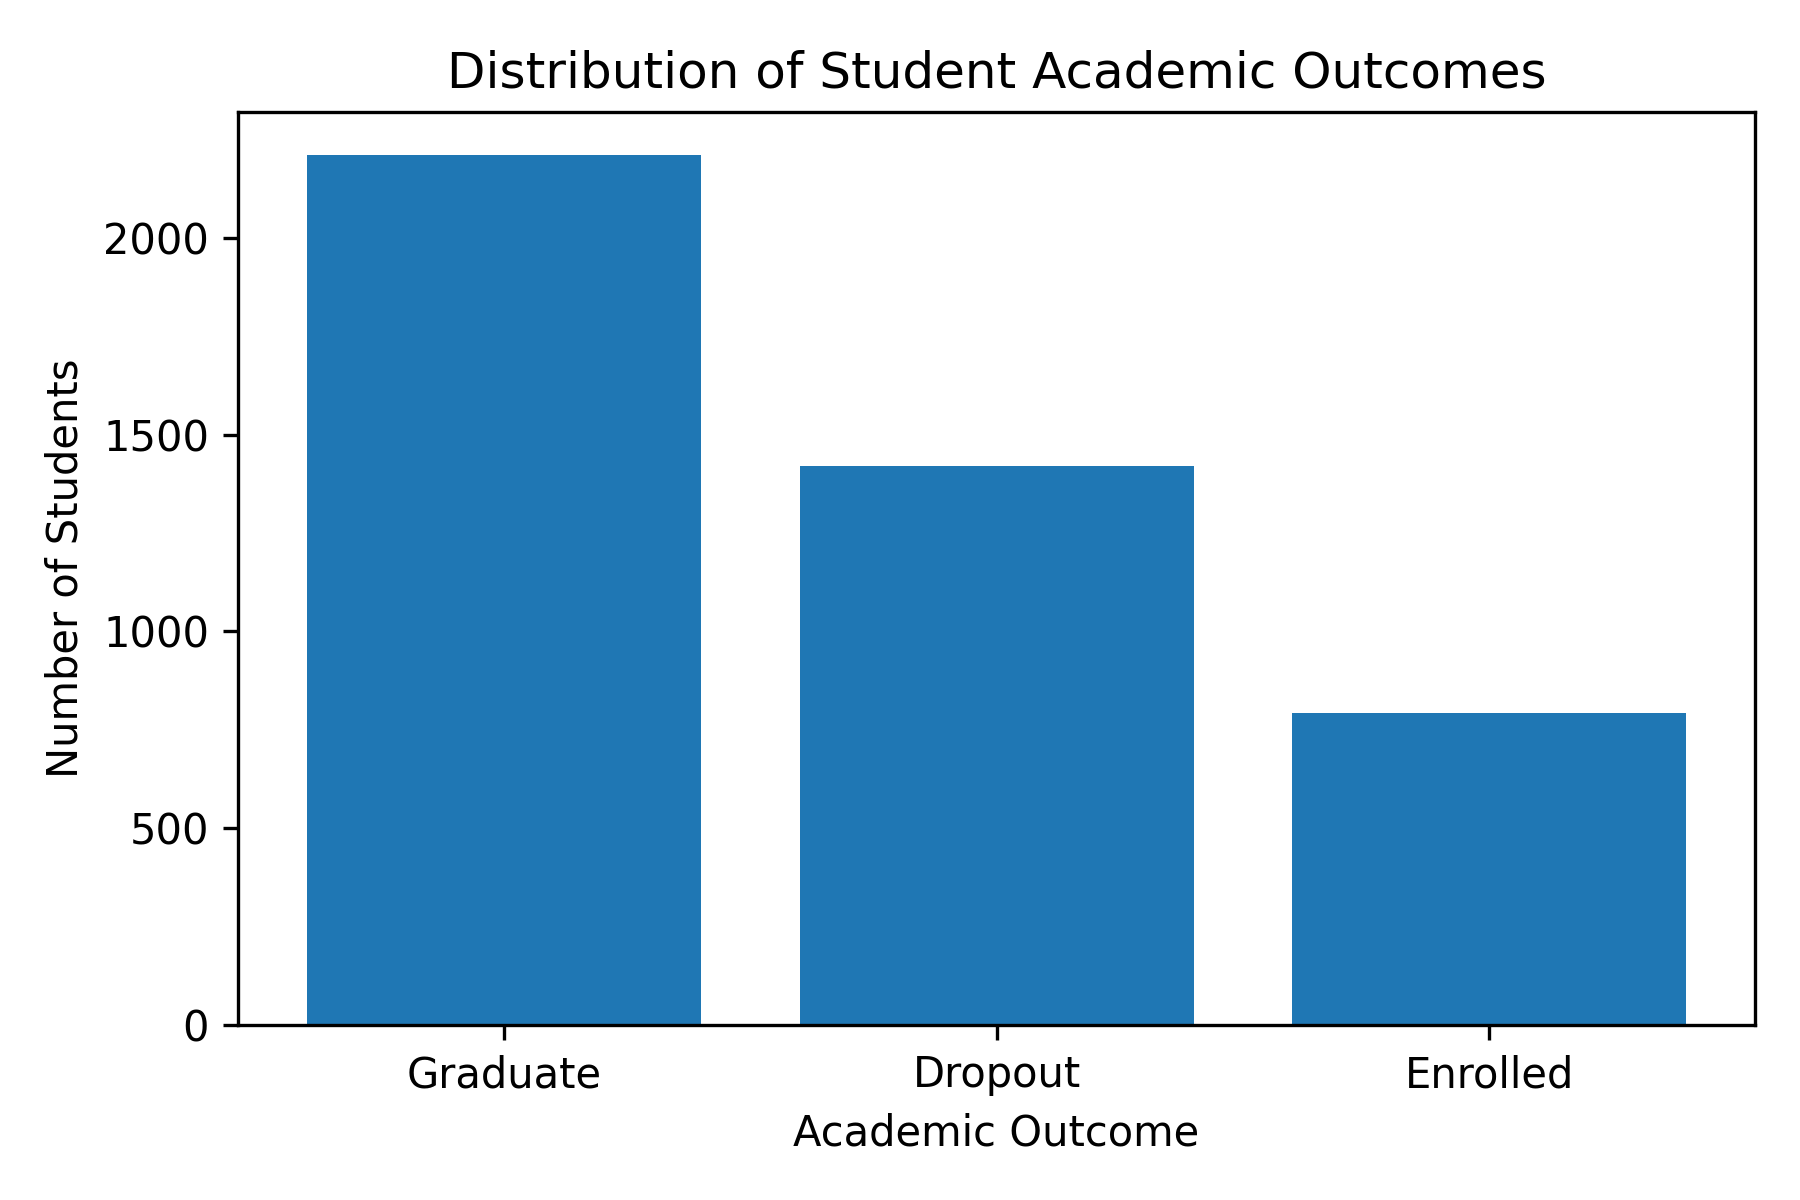
\includegraphics[width=0.70\linewidth]{figures/target_distribution.png}
    \caption{Distribution of academic outcome labels in the dataset. The \textit{Graduate} class is the largest class, while \textit{Enrolled} is the smallest, motivating the use of macro-averaged evaluation metrics.}
    \label{fig:target_distribution}
\end{figure}

\subsection{Selecting the number of student clusters}

To select the number of K-Means clusters, I evaluated \(k=2\) through \(k=10\) using the Elbow Method and Silhouette Score. As shown in Figure~\ref{fig:kmeans_selection}, the inertia decreases sharply from \(k=2\) to \(k=3\), after which improvements become more gradual. The silhouette score also reaches its highest value at \(k=3\). Based on these results, I selected \(k=3\) for the student segmentation step.

\begin{figure}[t]
    \centering
    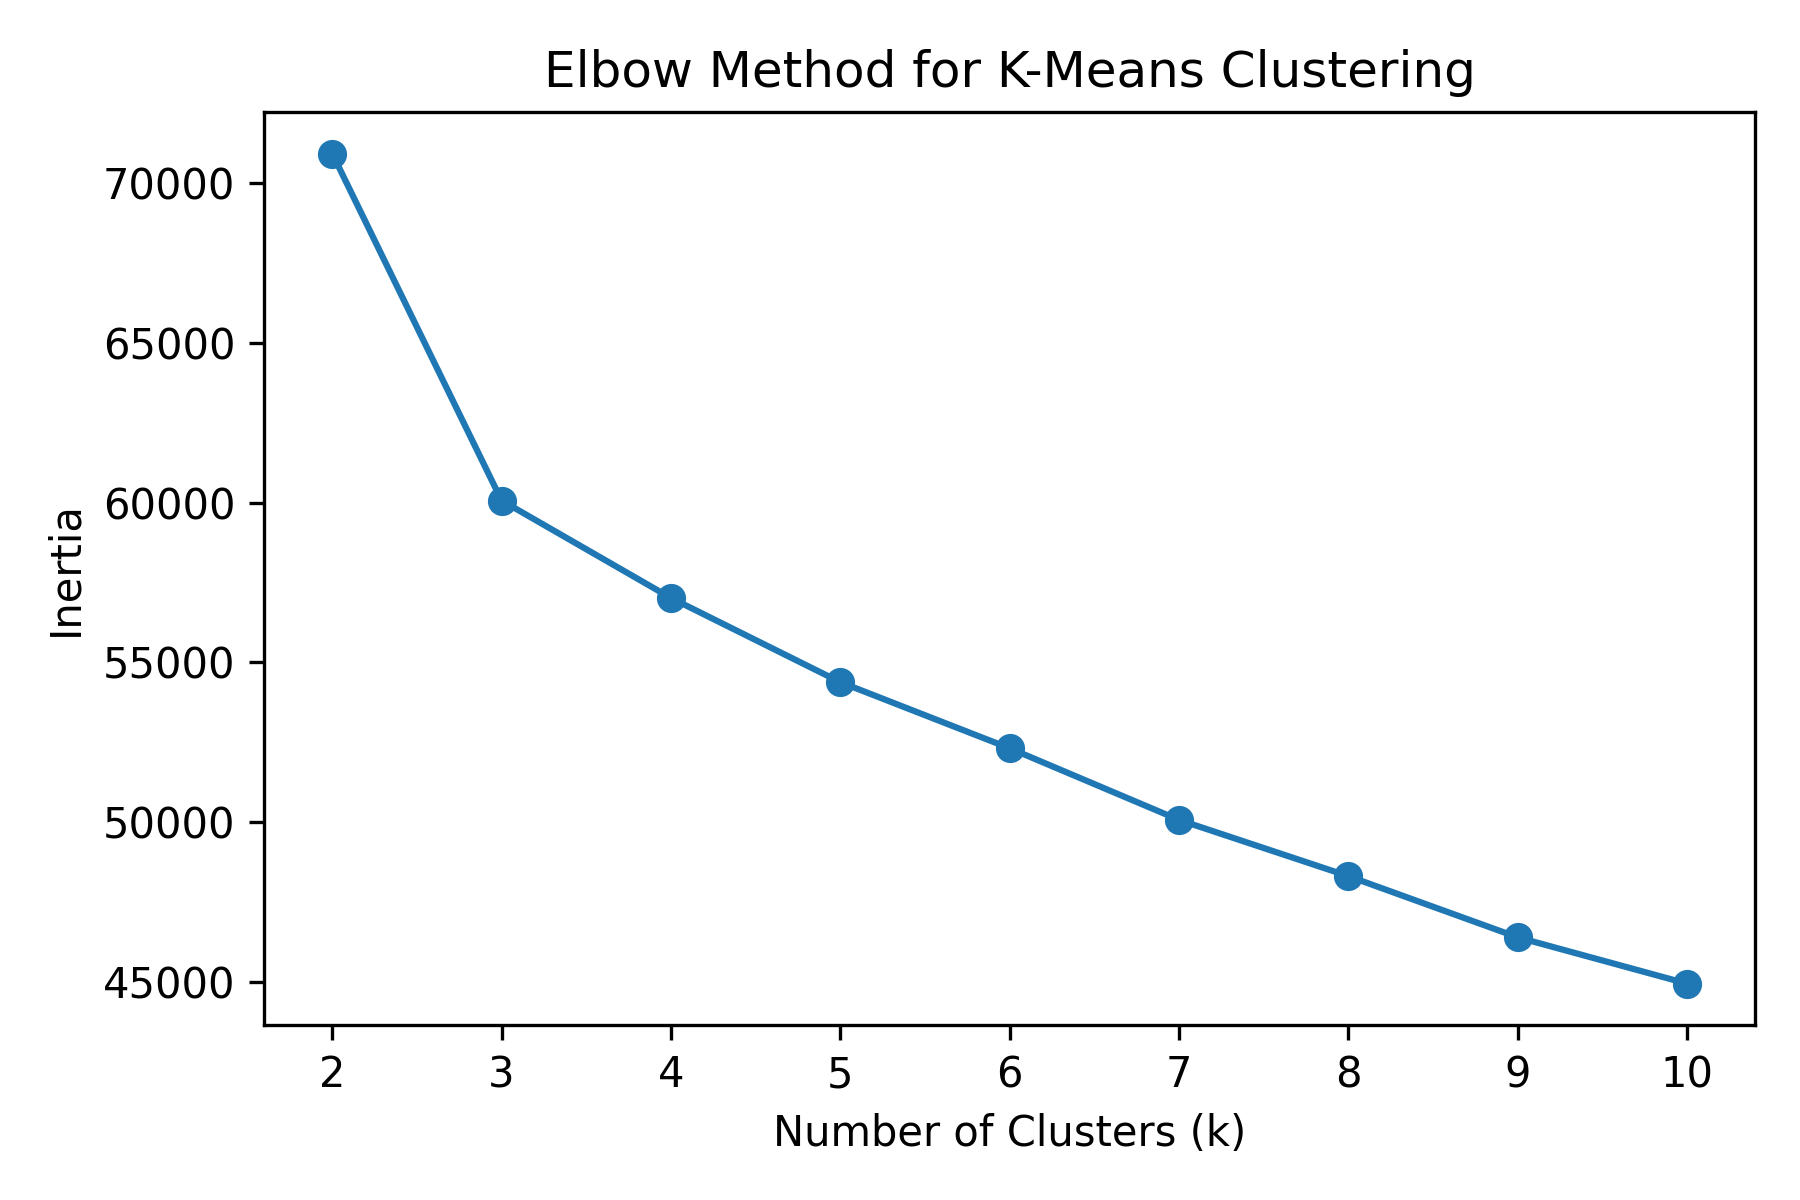
\includegraphics[width=0.48\linewidth]{figures/kmeans_elbow.png}
    \hfill
    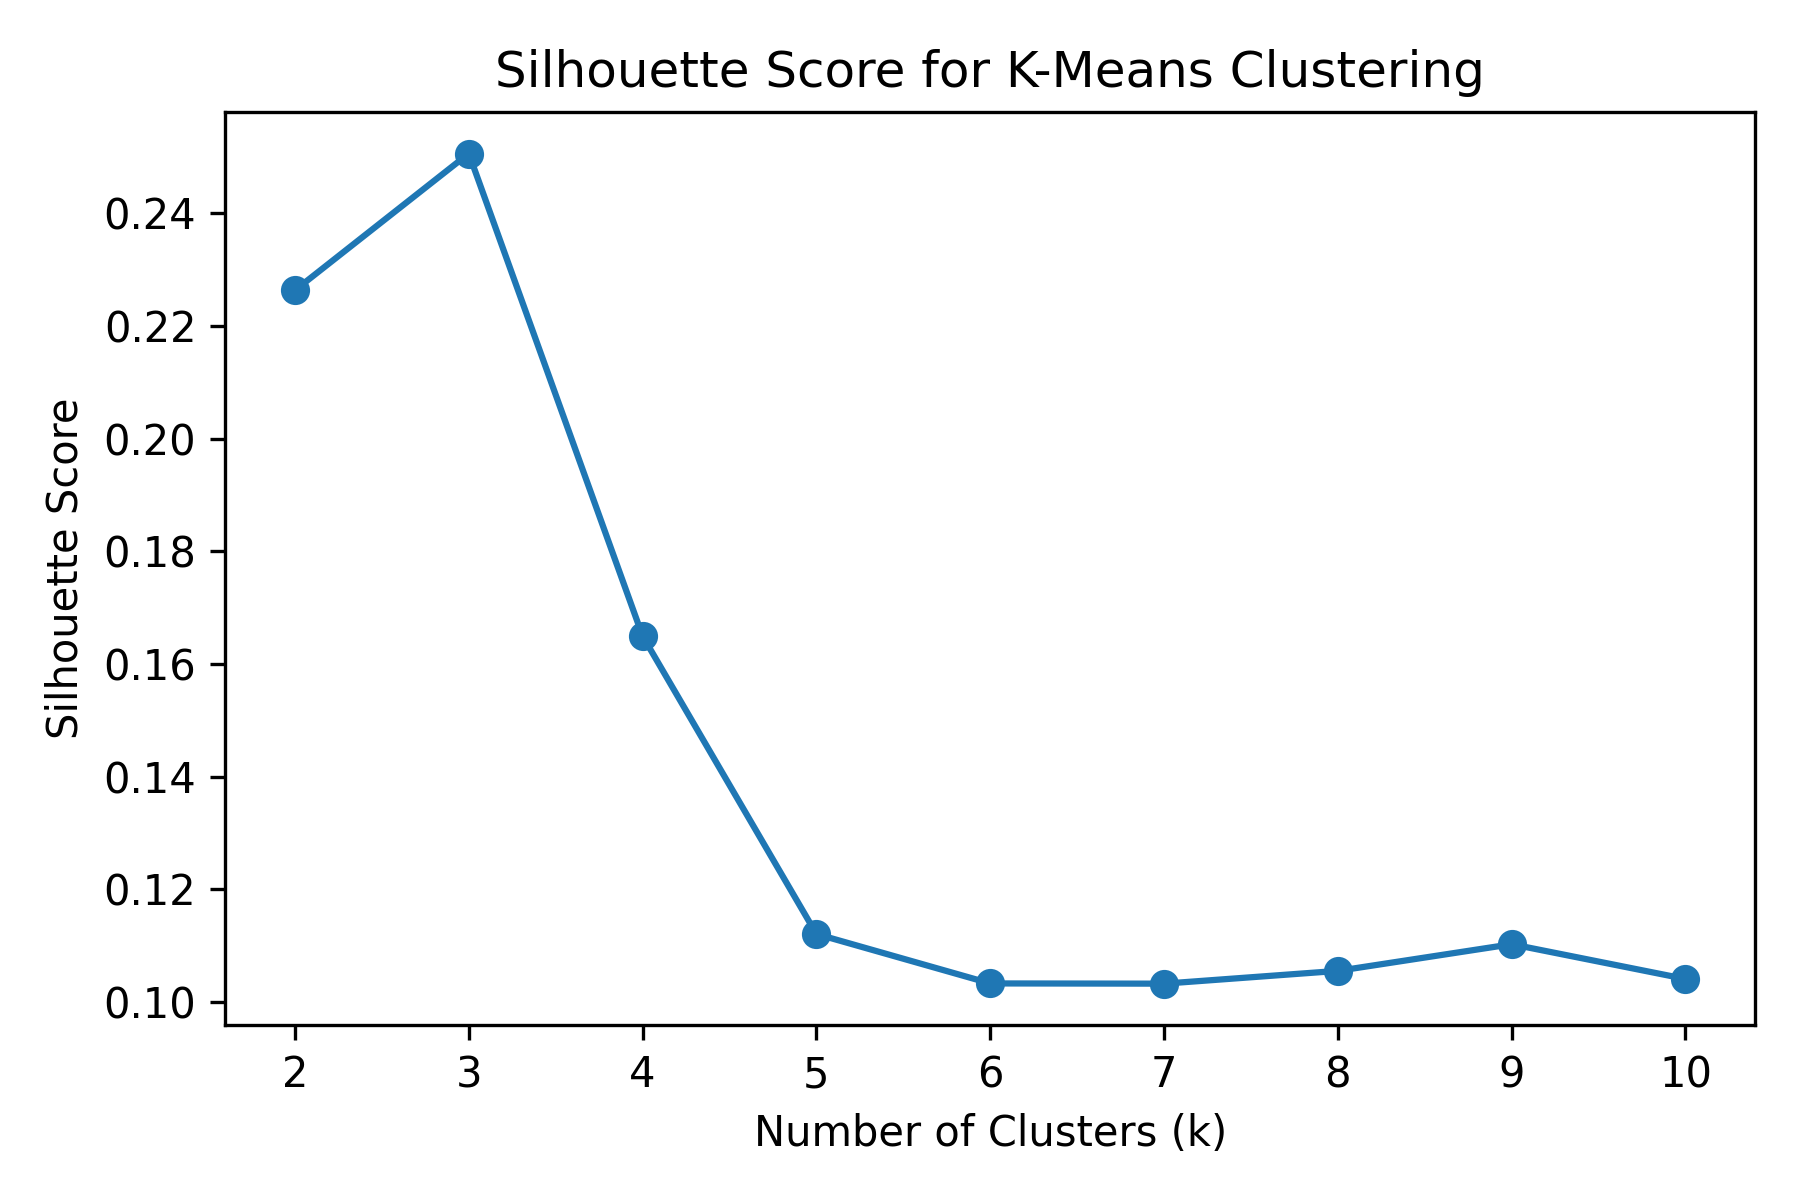
\includegraphics[width=0.48\linewidth]{figures/kmeans_silhouette.png}
    \caption{Selection of the number of K-Means clusters. The Elbow Method shows a large early reduction in inertia around \(k=3\), and the Silhouette Score is highest at \(k=3\).}
    \label{fig:kmeans_selection}
\end{figure}

\subsection{Student cluster visualization}

After fitting K-Means with \(k=3\), I used PCA to project the preprocessed training data into two dimensions for visualization. This projection was used only for visualization and was not used for model training. Figure~\ref{fig:pca_clusters} shows that the clusters are partially separated in the reduced feature space. Although PCA compresses a high-dimensional one-hot encoded feature matrix into only two dimensions, the visualization still suggests that K-Means captures meaningful structure in the student population.

\begin{figure}[t]
    \centering
    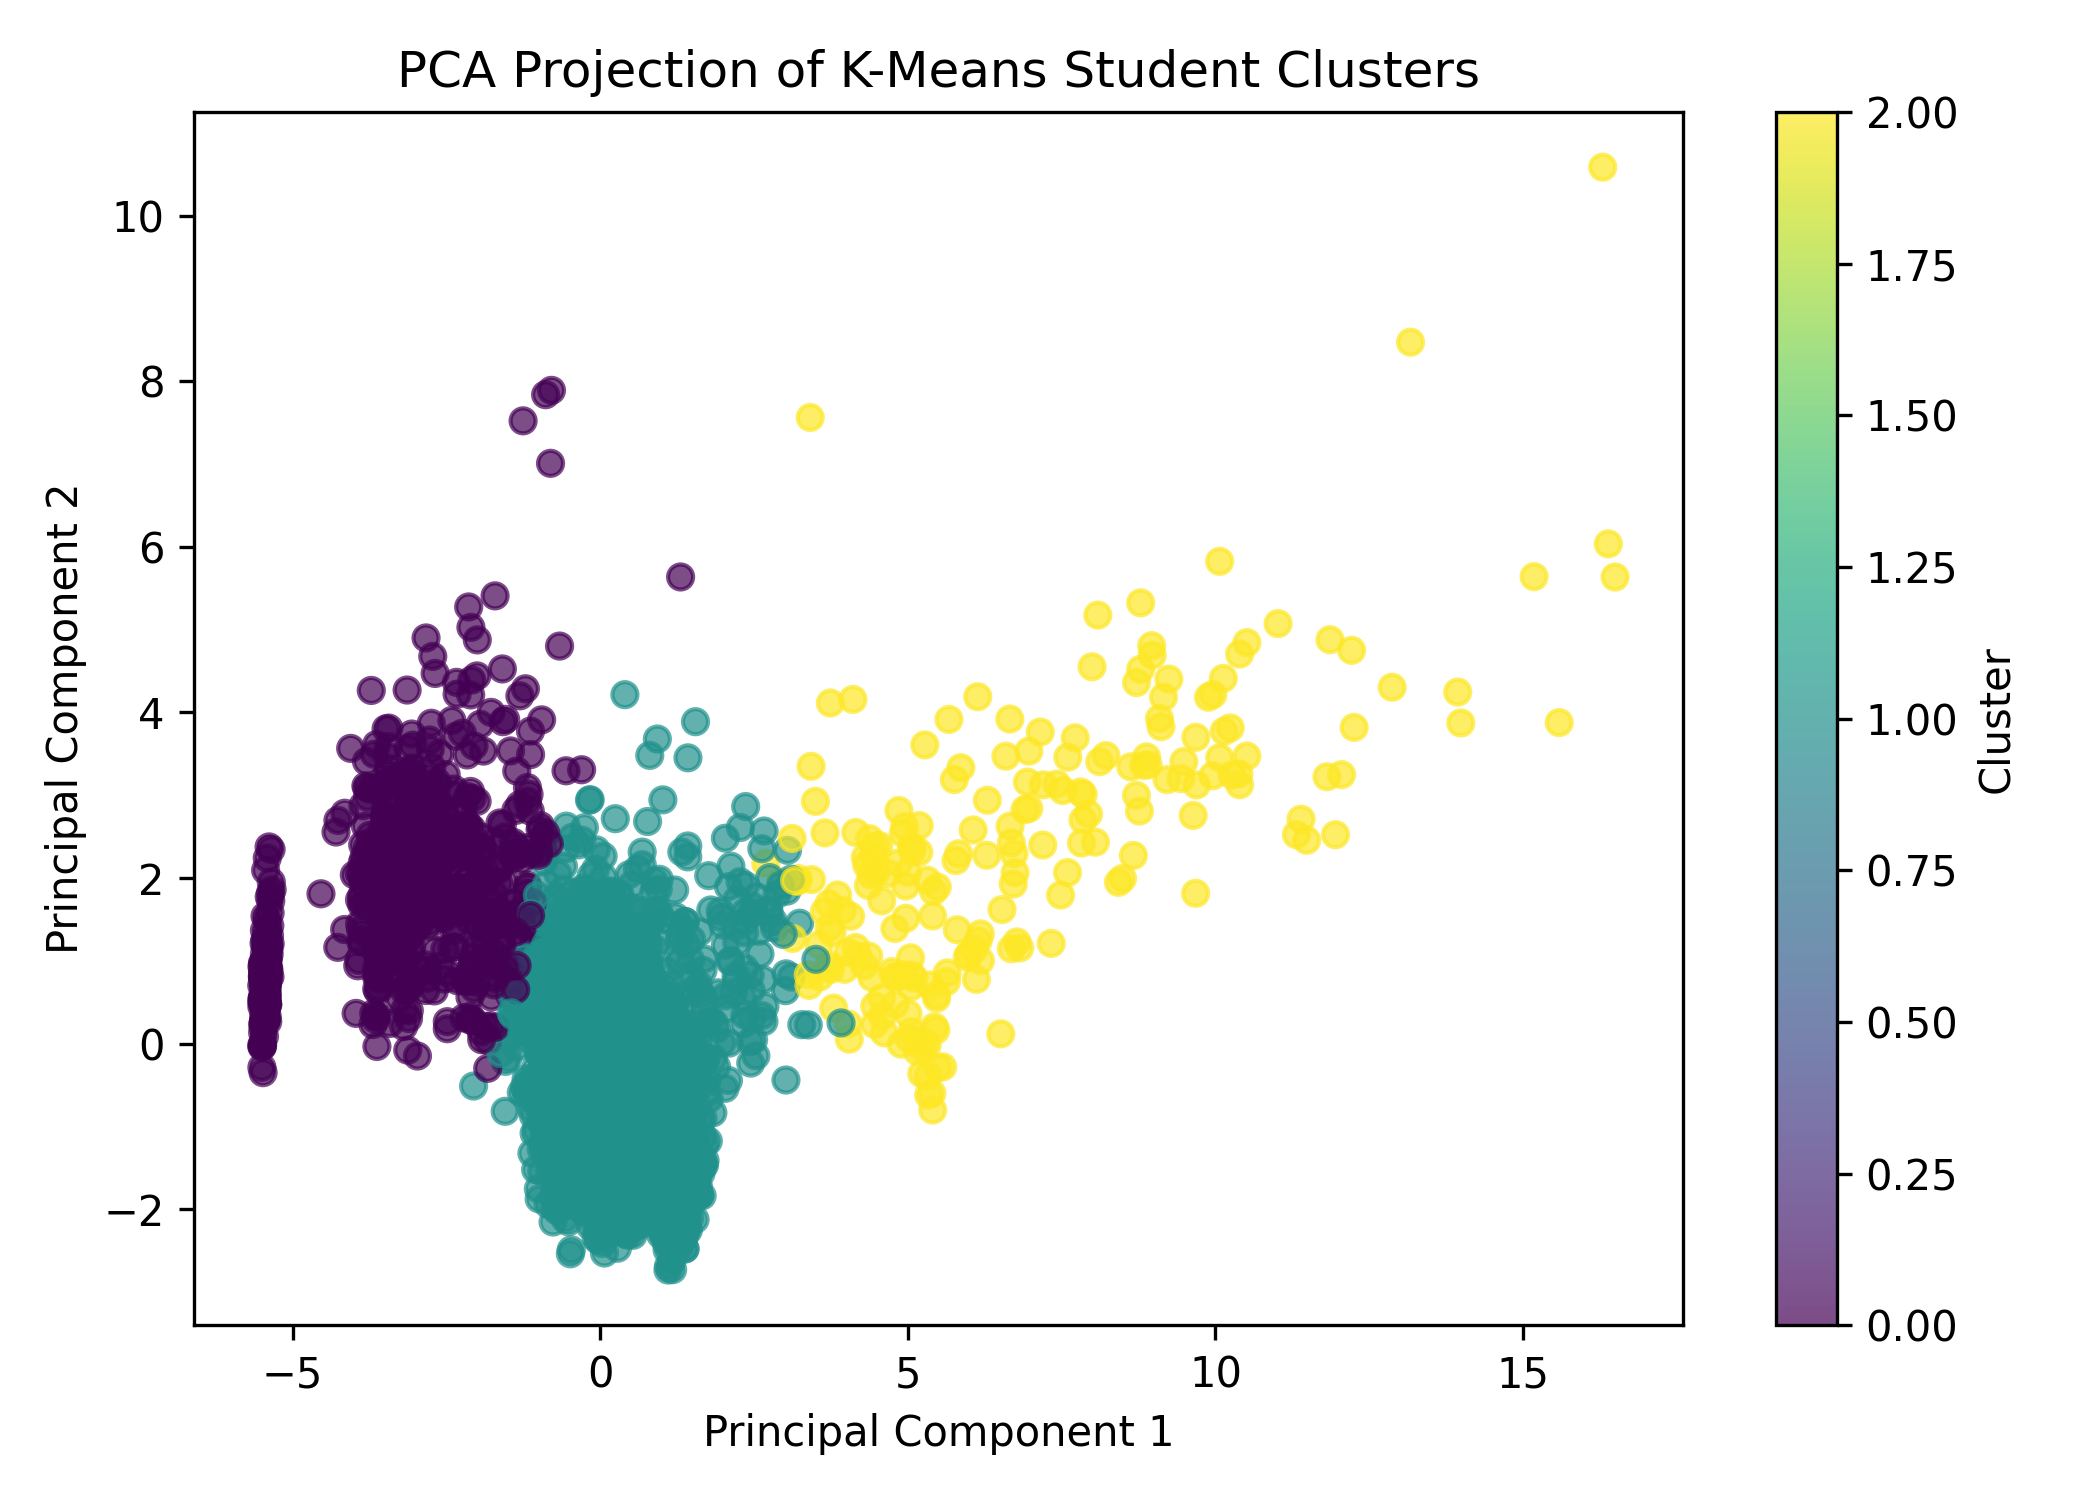
\includegraphics[width=0.75\linewidth]{figures/pca_clusters.png}
    \caption{PCA projection of K-Means student clusters. The visualization suggests that the preprocessed feature space contains separable student profiles, although the projection is only a two-dimensional approximation.}
    \label{fig:pca_clusters}
\end{figure}

\subsection{Cluster interpretation}

The K-Means clusters reveal meaningful differences in academic outcomes. Table~\ref{tab:cluster_outcomes} shows the distribution of target labels within each cluster. Cluster 0 is a clear high-risk segment: 82.0\% of students in this cluster are labeled as \textit{Dropout}, while only 9.6\% are labeled as \textit{Graduate}. In contrast, Clusters 1 and 2 are majority-graduate groups, with graduation proportions of 59.4\% and 60.6\%, respectively.

\begin{table}[t]
\centering
\caption{Academic outcome distribution within each K-Means cluster.}
\label{tab:cluster_outcomes}
\begin{tabular}{lrrr}
\toprule
Cluster & Dropout & Enrolled & Graduate \\
\midrule
0 & 0.820 & 0.084 & 0.096 \\
1 & 0.199 & 0.207 & 0.594 \\
2 & 0.245 & 0.148 & 0.606 \\
\bottomrule
\end{tabular}
\end{table}

The cluster profiles in Table~\ref{tab:cluster_profiles} help explain these outcome differences. Cluster 0 has extremely low averages for first-semester and second-semester curricular units approved, as well as a very low second-semester grade. This suggests that the cluster represents students who made little academic progress during the observed period. Cluster 1 consists of younger students with relatively strong academic progress, higher scholarship rates, and high tuition payment status. Cluster 2 contains older students with the highest number of curricular units approved and strong semester grades.

\begin{table}[t]
\centering
\caption{Selected feature averages for each K-Means cluster.}
\label{tab:cluster_profiles}
\resizebox{\textwidth}{!}{
\begin{tabular}{lrrrrrrr}
\toprule
Cluster & Age & Tuition Paid & Debtor & Scholarship & 1st Sem Approved & 2nd Sem Approved & 2nd Sem Grade \\
\midrule
0 & 26.099 & 0.717 & 0.189 & 0.103 & 0.318 & 0.085 & 0.573 \\
1 & 22.066 & 0.921 & 0.087 & 0.303 & 5.259 & 5.088 & 12.472 \\
2 & 28.778 & 0.912 & 0.148 & 0.111 & 11.662 & 10.093 & 12.728 \\
\bottomrule
\end{tabular}
}
\end{table}

\begin{figure}[t]
    \centering
    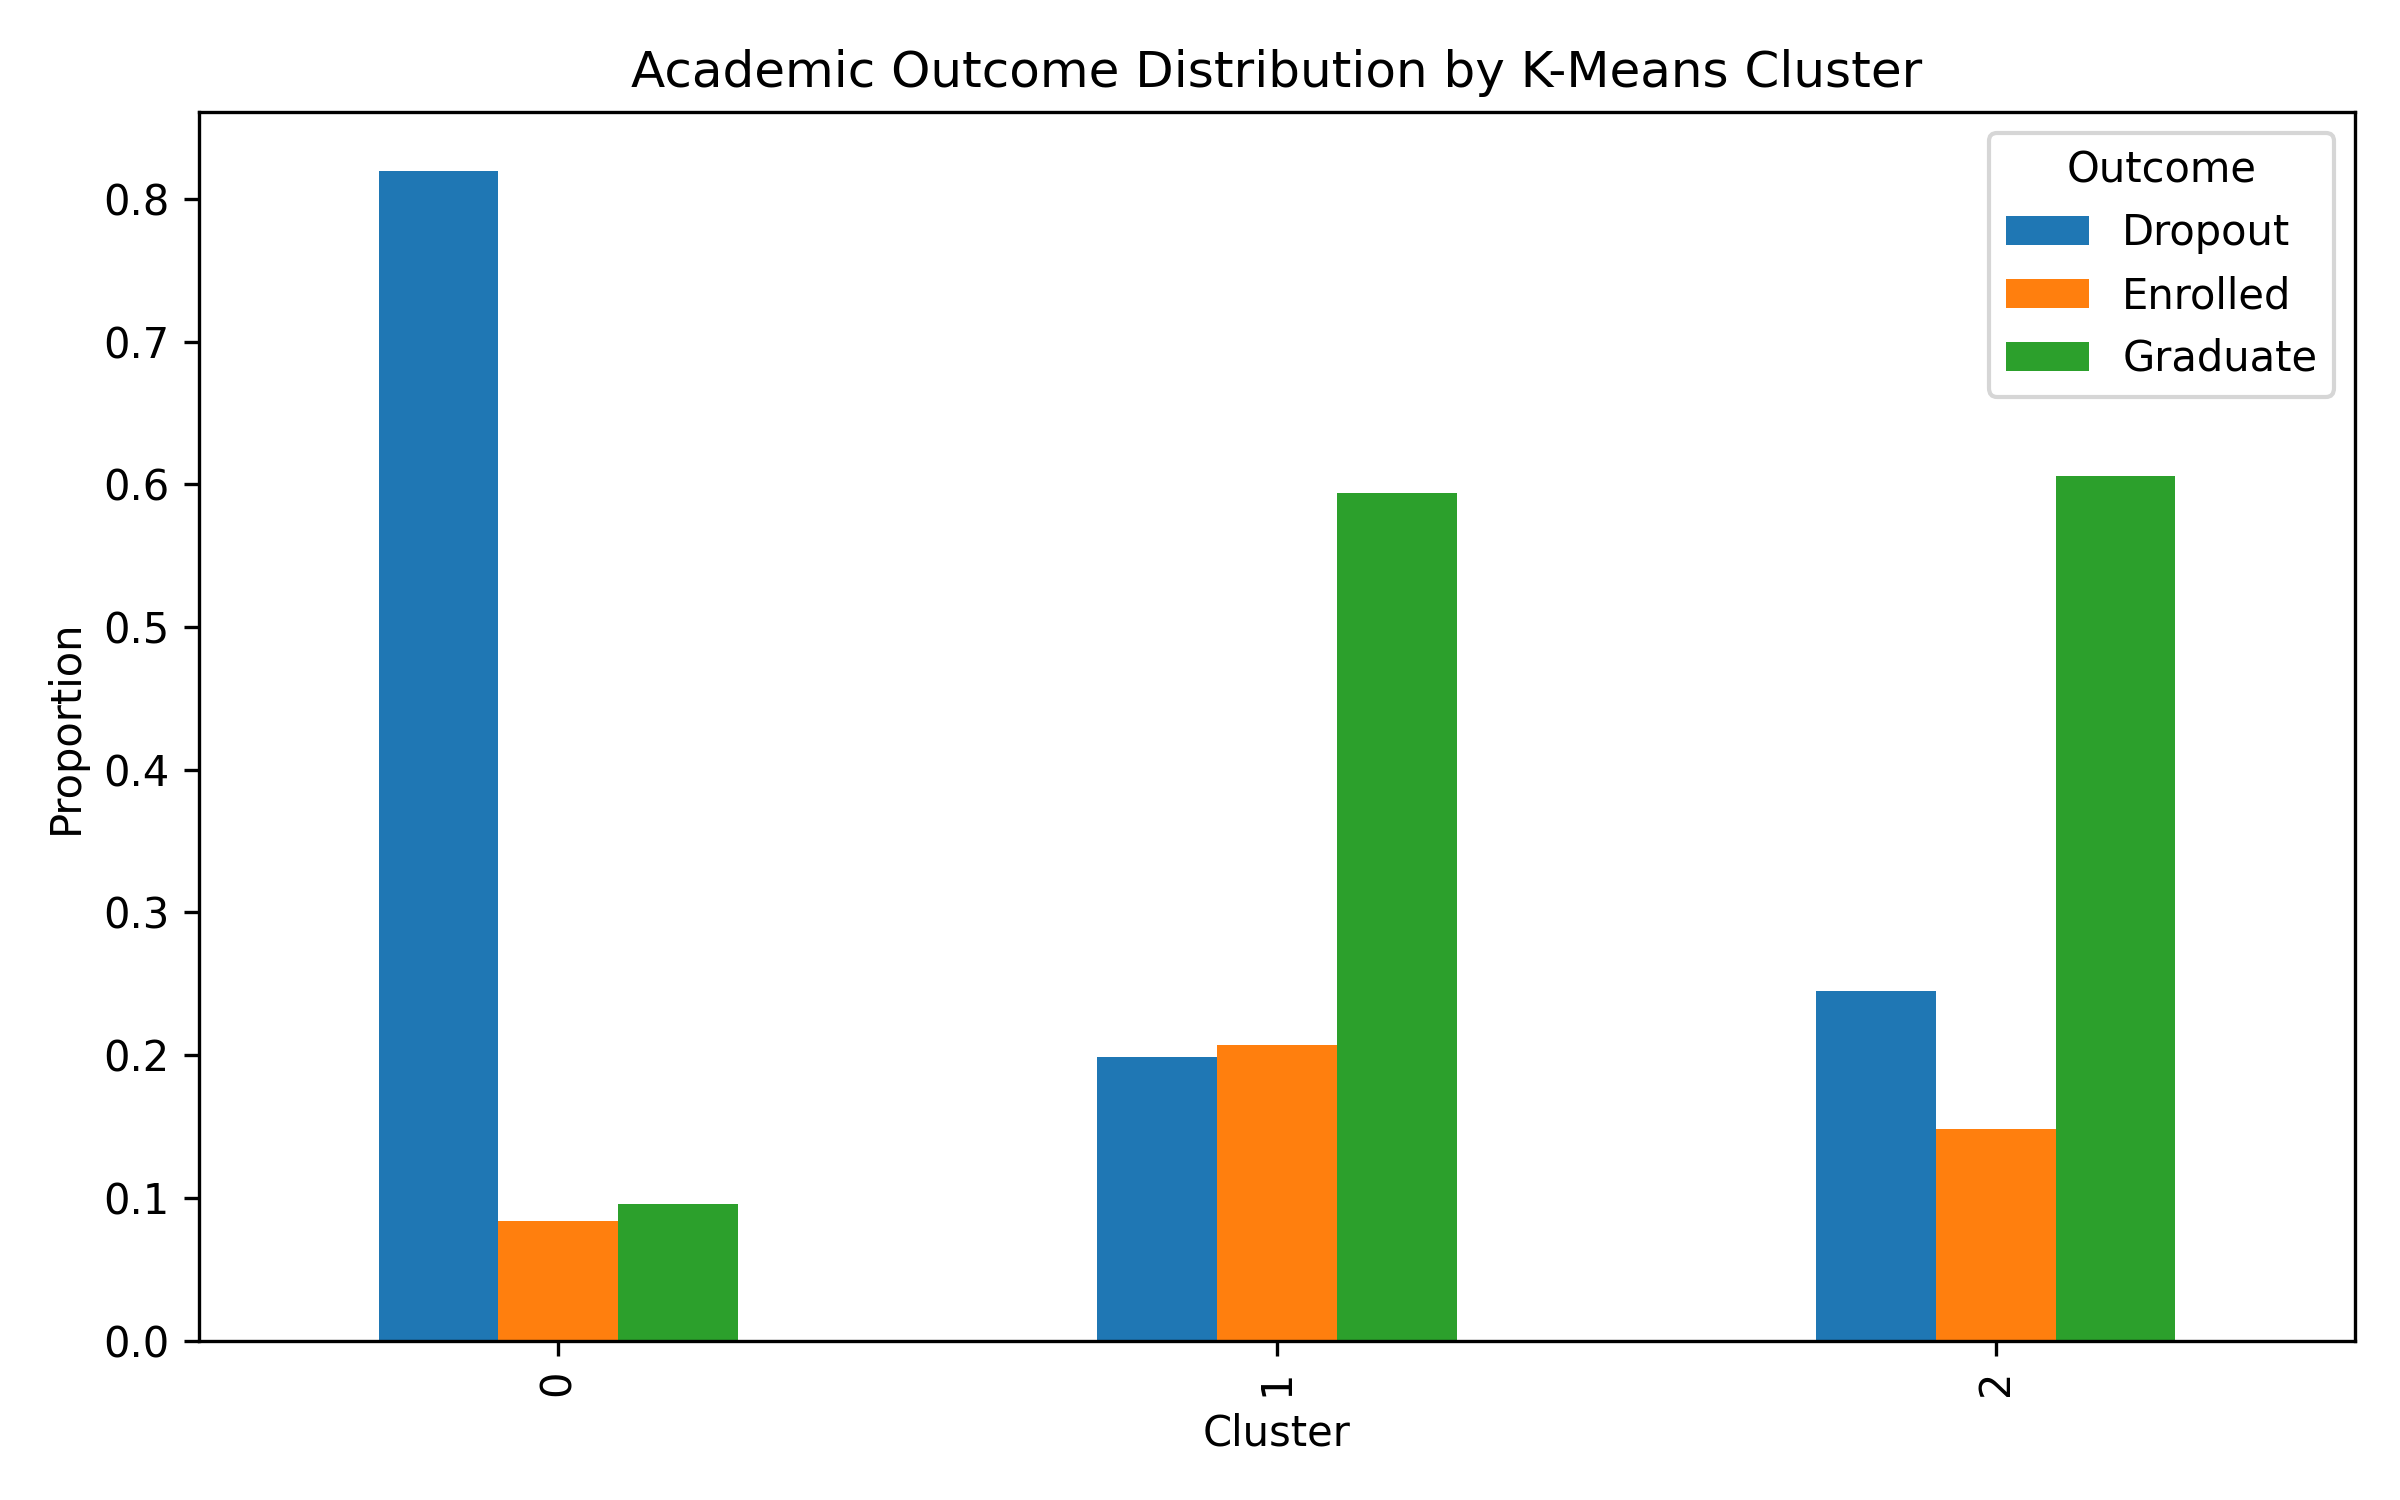
\includegraphics[width=0.78\linewidth]{figures/cluster_outcome_distribution.png}
    \caption{Academic outcome proportions by K-Means cluster. Cluster 0 is dominated by dropout outcomes, while Clusters 1 and 2 contain majority-graduate student profiles.}
    \label{fig:cluster_outcomes}
\end{figure}

\subsection{Supervised classification results}

Table~\ref{tab:model_results} compares the baseline and cluster-augmented versions of Logistic Regression, Random Forest, and Extra Trees. The baseline Random Forest achieved the highest overall accuracy, 0.7605, and the highest macro ROC-AUC, 0.8902. This suggests that the nonlinear ensemble model was best at separating the three classes overall. However, Logistic Regression achieved the highest macro F1-score, 0.6852, indicating a more balanced trade-off across the imbalanced classes.

Adding cluster labels as additional features did not consistently improve predictive performance. The cluster-augmented Random Forest had the same accuracy as the baseline Random Forest but slightly lower macro F1 and macro ROC-AUC. Extra Trees improved slightly when cluster labels were added, increasing macro F1 from 0.6402 to 0.6505 and macro ROC-AUC from 0.8741 to 0.8783. Overall, the results suggest that K-Means cluster labels can add some useful information for certain models, but the original academic and enrollment features already contain most of the predictive signal.

\begin{table}[t]
\centering
\caption{Performance comparison of baseline and cluster-augmented models on the test set.}
\label{tab:model_results}
\resizebox{\textwidth}{!}{
\begin{tabular}{llrrrrr}
\toprule
Model & Pipeline & Accuracy & Macro Precision & Macro Recall & Macro F1 & Macro ROC-AUC \\
\midrule
Logistic Regression & Baseline & 0.7232 & 0.6921 & 0.6964 & 0.6852 & 0.8775 \\
Random Forest & Baseline & 0.7605 & 0.7036 & 0.6610 & 0.6698 & 0.8902 \\
Extra Trees & Baseline & 0.7401 & 0.6772 & 0.6332 & 0.6402 & 0.8741 \\
Logistic Regression & Cluster-Augmented & 0.7198 & 0.6907 & 0.6925 & 0.6814 & 0.8779 \\
Random Forest & Cluster-Augmented & 0.7605 & 0.7001 & 0.6555 & 0.6626 & 0.8889 \\
Extra Trees & Cluster-Augmented & 0.7469 & 0.6872 & 0.6419 & 0.6505 & 0.8783 \\
\bottomrule
\end{tabular}
}
\end{table}

\begin{figure}[t]
    \centering
    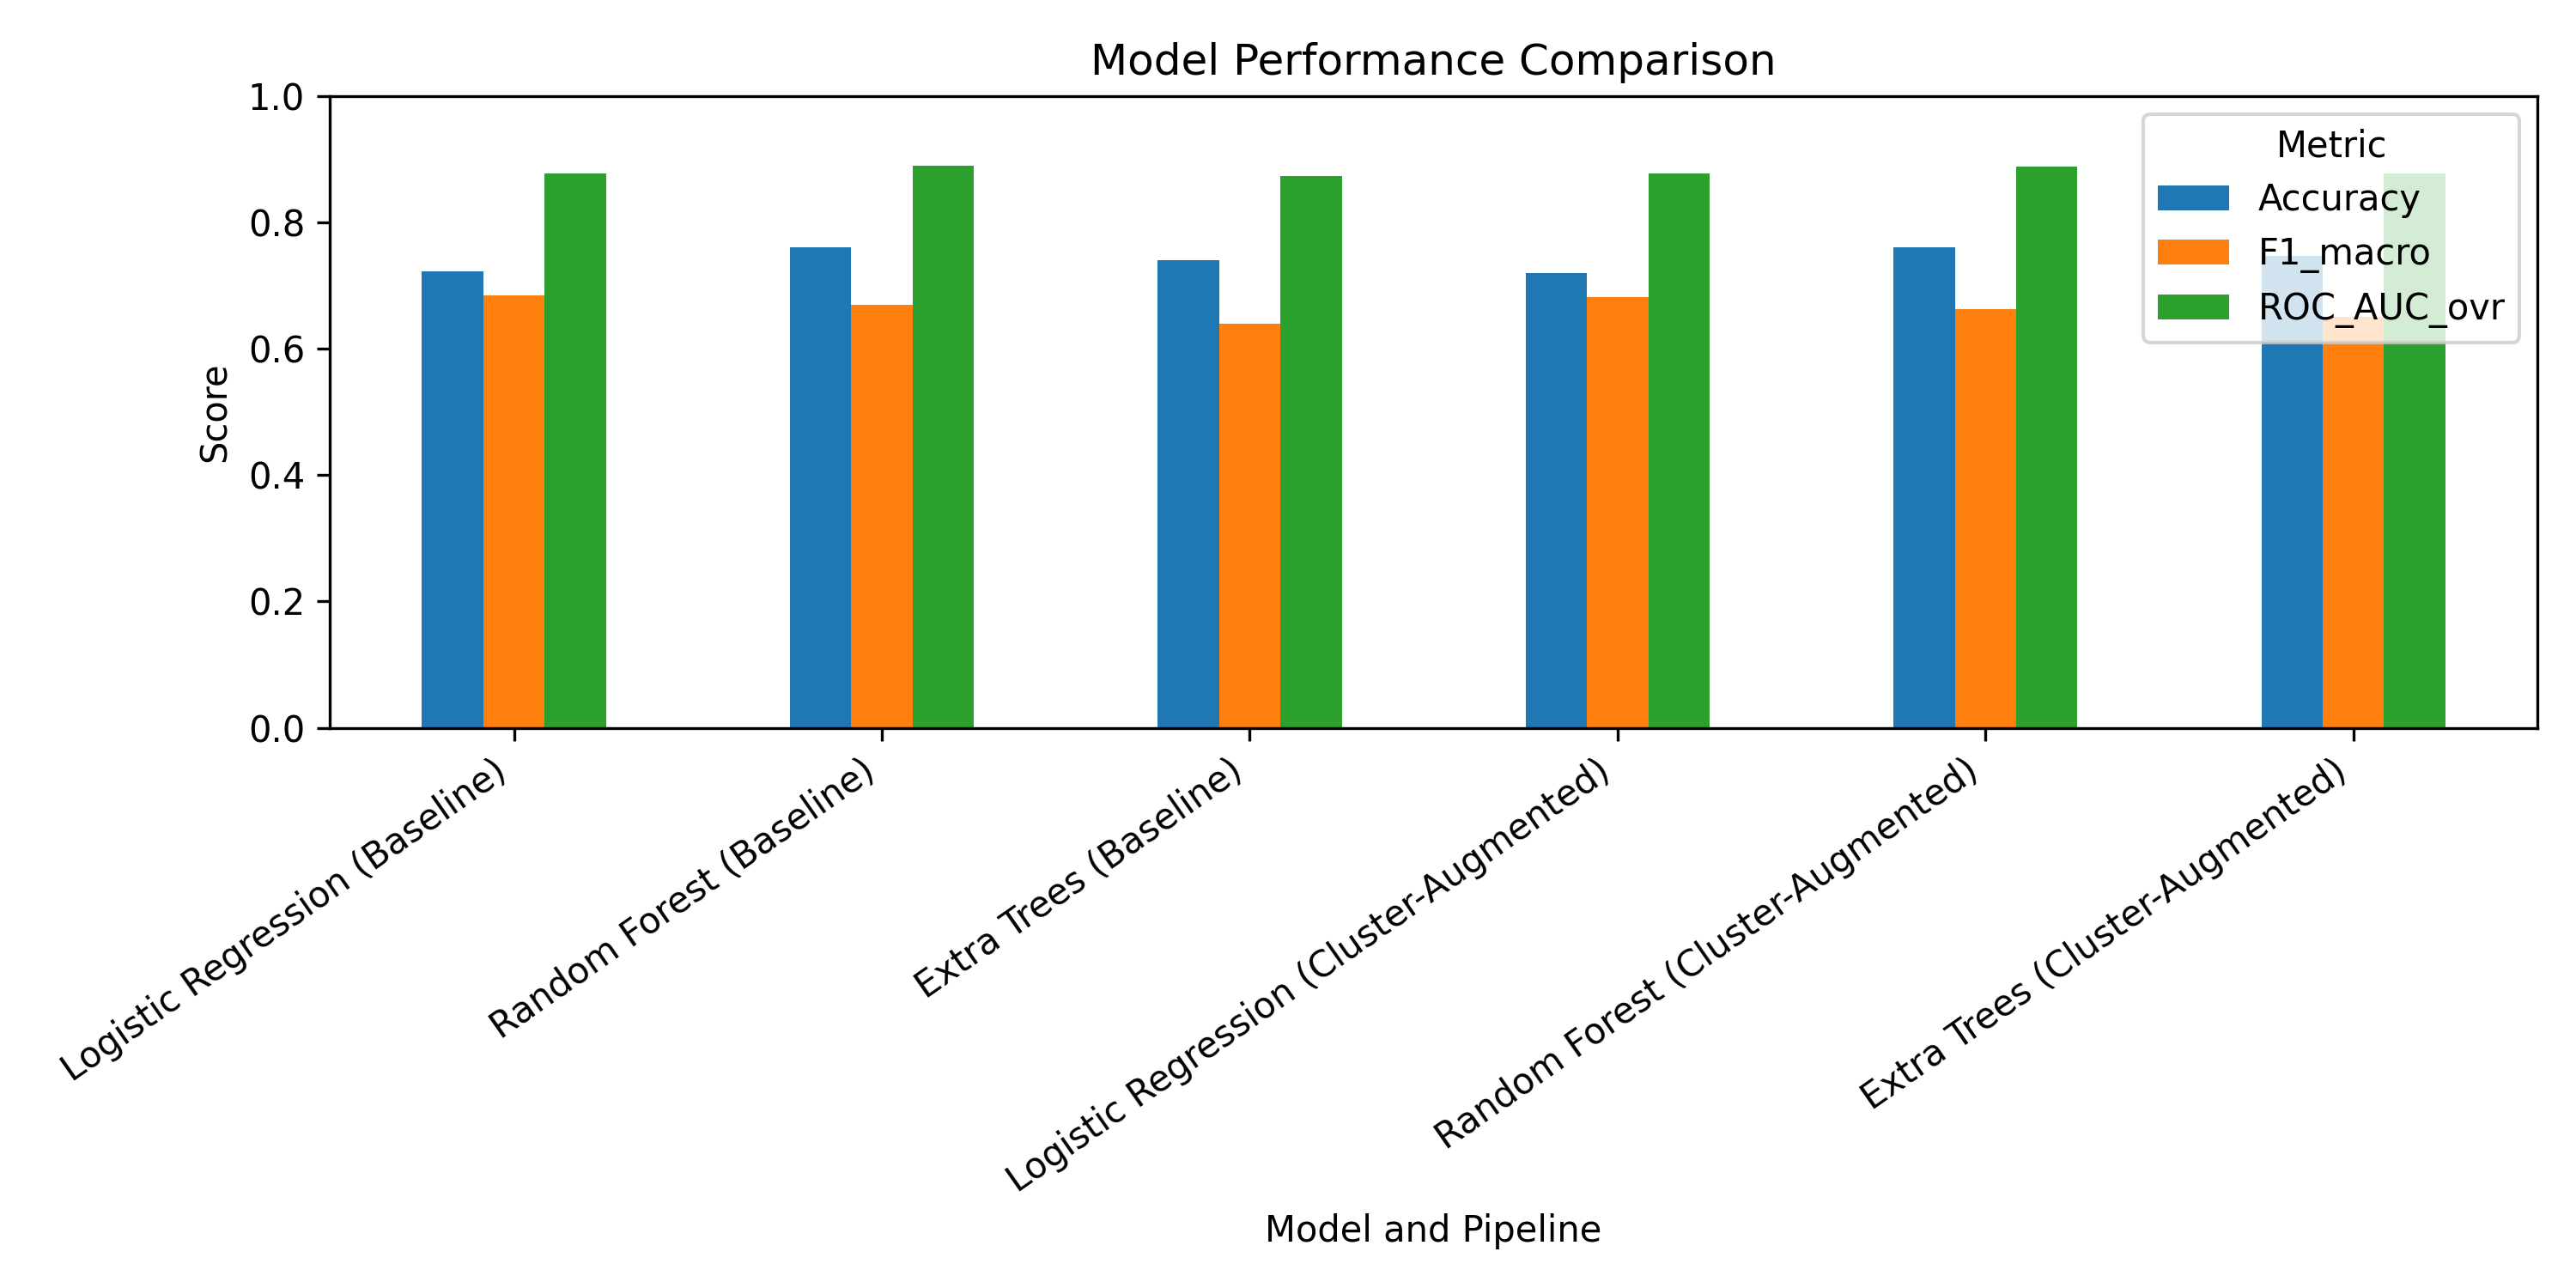
\includegraphics[width=0.90\linewidth]{figures/model_comparison.png}
    \caption{Comparison of model performance across baseline and cluster-augmented pipelines. Random Forest achieved the strongest accuracy and macro ROC-AUC, while Logistic Regression achieved the strongest macro F1-score.}
    \label{fig:model_comparison}
\end{figure}

\subsection{Class-level error analysis}

The normalized confusion matrices in Figure~\ref{fig:confusion_matrices} provide a more detailed view of model behavior. Logistic Regression performs better on the minority \textit{Enrolled} class than Random Forest, which helps explain why it obtains the strongest macro F1-score. Random Forest performs especially well on the \textit{Graduate} class, correctly identifying 94\% of graduate students, but it struggles more with the \textit{Enrolled} class. This illustrates why accuracy alone is not sufficient for this problem: a model can obtain strong overall accuracy while still underperforming on the smaller class.

\begin{figure}[t]
    \centering
    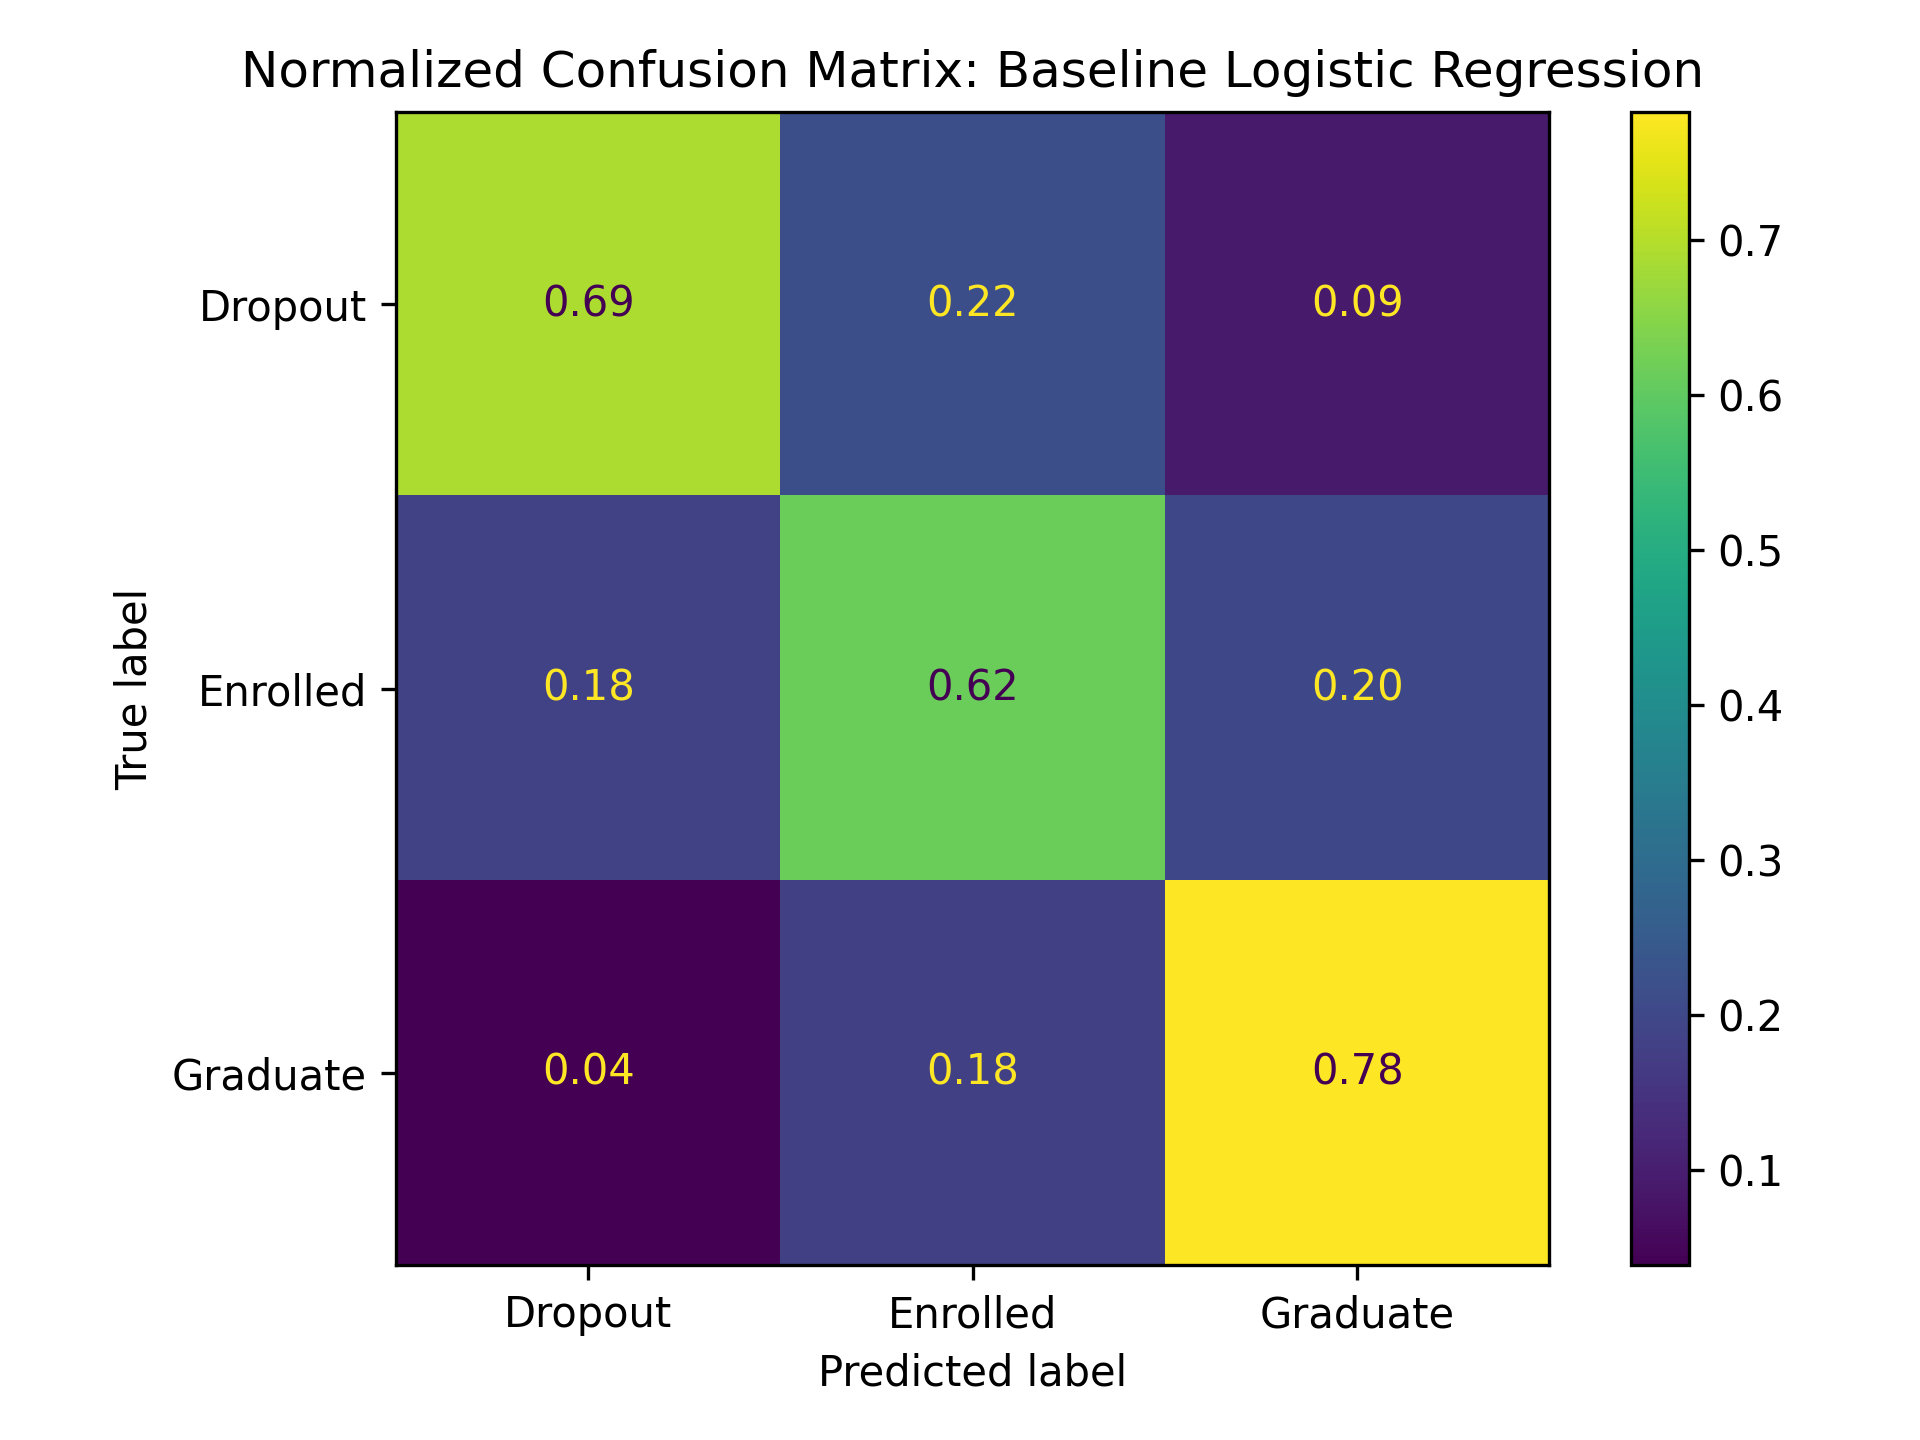
\includegraphics[width=0.48\linewidth]{figures/confusion_matrix_logistic_regression.png}
    \hfill
    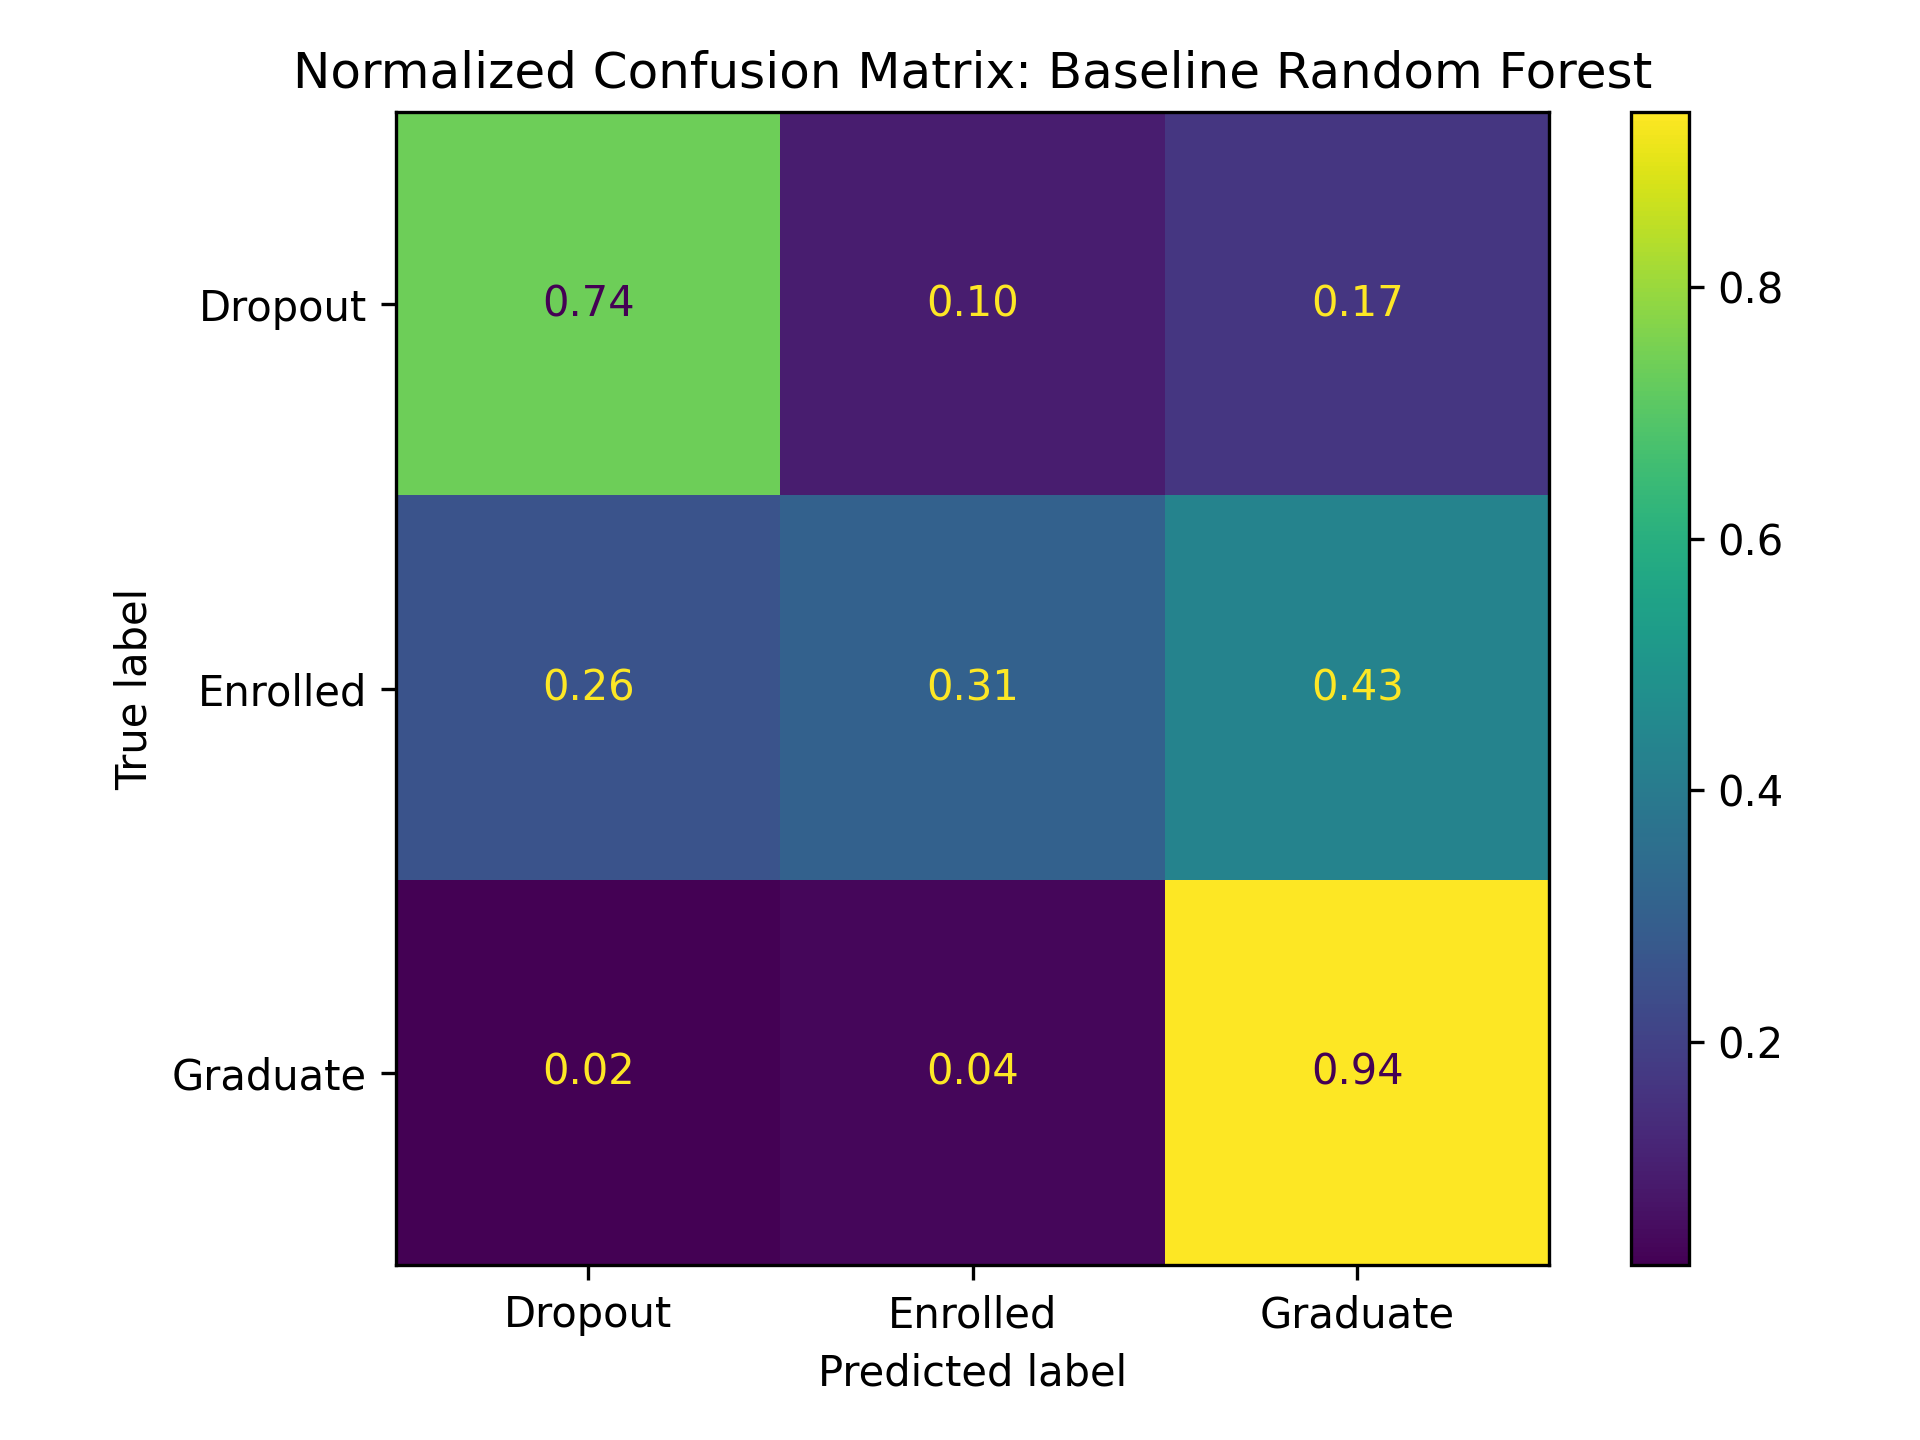
\includegraphics[width=0.48\linewidth]{figures/confusion_matrix_random_forest.png}
    \caption{Normalized confusion matrices for baseline Logistic Regression and baseline Random Forest. Logistic Regression is more balanced across classes, while Random Forest is strongest on the majority \textit{Graduate} class.}
    \label{fig:confusion_matrices}
\end{figure}

The one-vs-rest ROC curves for Random Forest are shown in Figure~\ref{fig:roc_rf}. The model separates \textit{Dropout} and \textit{Graduate} students more effectively than the \textit{Enrolled} class. This is consistent with the confusion matrix results and reflects the difficulty of predicting students who remain enrolled without graduating or dropping out.

\begin{figure}[t]
    \centering
    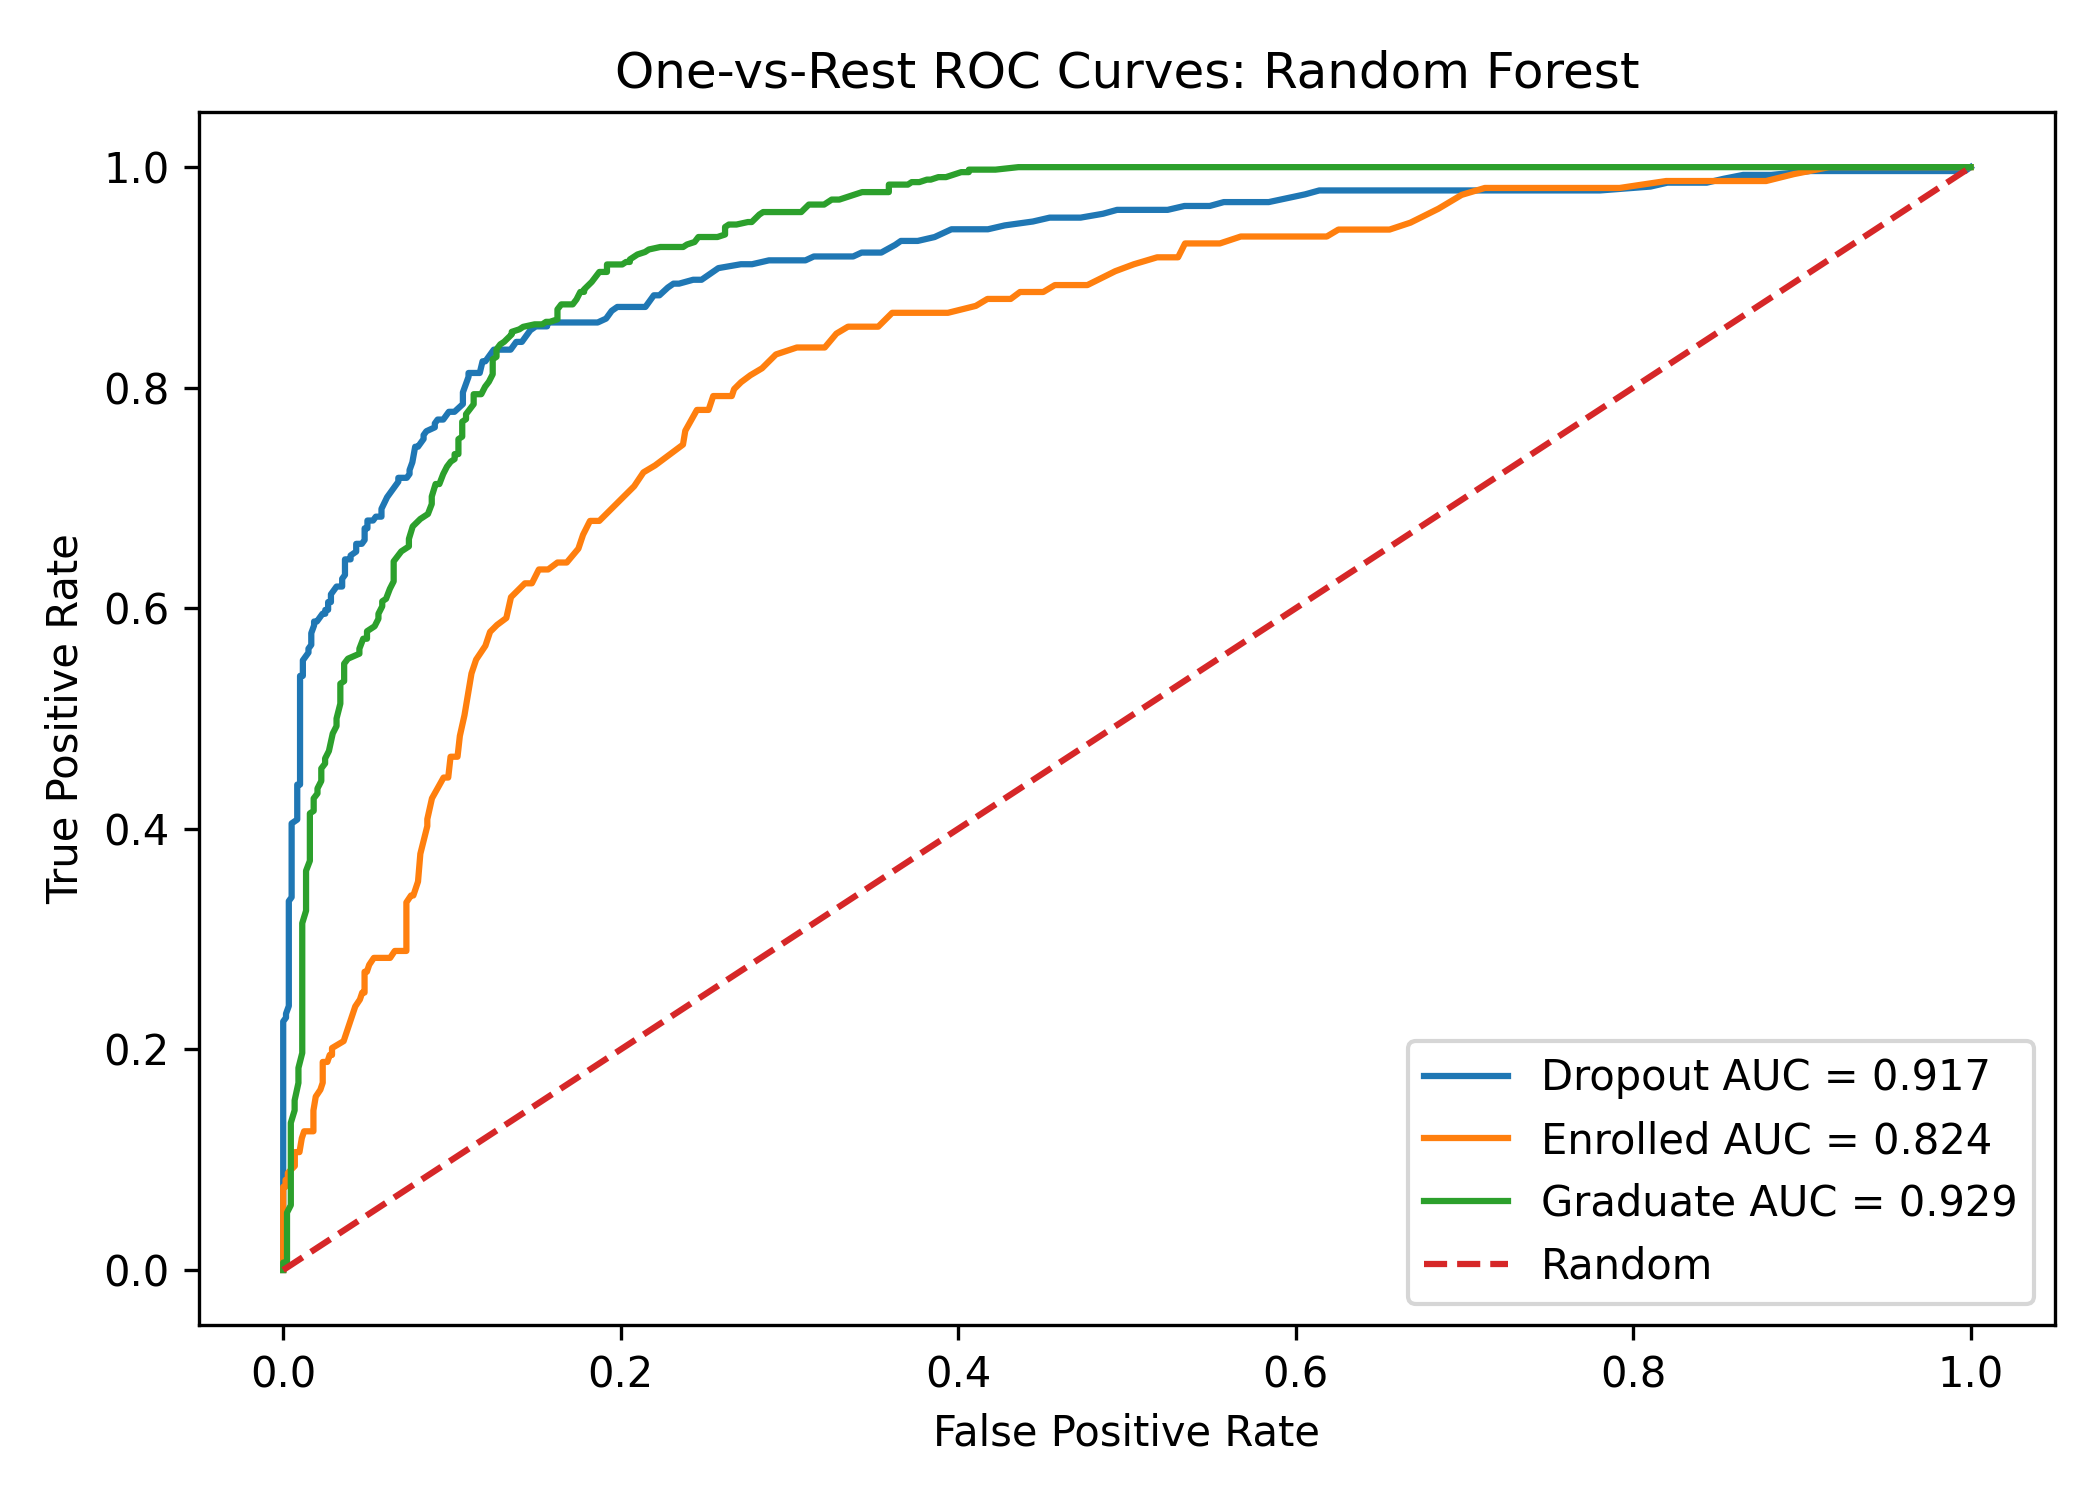
\includegraphics[width=0.78\linewidth]{figures/roc_curves_random_forest.png}
    \caption{One-vs-rest ROC curves for the baseline Random Forest model. The model achieves strong separability overall, but the \textit{Enrolled} class remains more difficult than the \textit{Dropout} and \textit{Graduate} classes.}
    \label{fig:roc_rf}
\end{figure}

\subsection{Feature importance analysis}

To interpret the best-performing ensemble model, I extracted feature importance scores from the baseline Random Forest. The top features are shown in Table~\ref{tab:feature_importance} and Figure~\ref{fig:feature_importance}. The most important predictors are academic progress variables from the first and second semesters, including the number of curricular units approved and semester grades. This result is intuitive: students who approve more curricular units and earn stronger grades are more likely to persist and graduate, while students with little academic progress are more likely to drop out.

Financial and contextual variables also appear in the top rankings. Tuition payment status, GDP, unemployment rate, inflation rate, scholarship holder status, and application order all contribute to the model. However, their importance values are lower than those of direct academic performance variables. This suggests that early academic progress is the strongest signal for predicting final academic outcome, while socioeconomic and enrollment variables provide additional context.

\begin{table}[t]
\centering
\caption{Top 15 Random Forest feature importances.}
\label{tab:feature_importance}
\resizebox{\textwidth}{!}{
\begin{tabular}{lr}
\toprule
Feature & Importance \\
\midrule
Curricular units 2nd sem (approved) & 0.0996 \\
Curricular units 2nd sem (grade) & 0.0826 \\
Curricular units 1st sem (grade) & 0.0624 \\
Curricular units 1st sem (approved) & 0.0614 \\
Curricular units 2nd sem (evaluations) & 0.0455 \\
Curricular units 1st sem (evaluations) & 0.0407 \\
Age at enrollment & 0.0401 \\
Tuition fees up to date & 0.0295 \\
GDP & 0.0261 \\
Unemployment rate & 0.0257 \\
Inflation rate & 0.0236 \\
Curricular units 2nd sem (enrolled) & 0.0206 \\
Curricular units 1st sem (enrolled) & 0.0195 \\
Scholarship holder & 0.0167 \\
Application order & 0.0166 \\
\bottomrule
\end{tabular}
}
\end{table}

\begin{figure}[t]
    \centering
    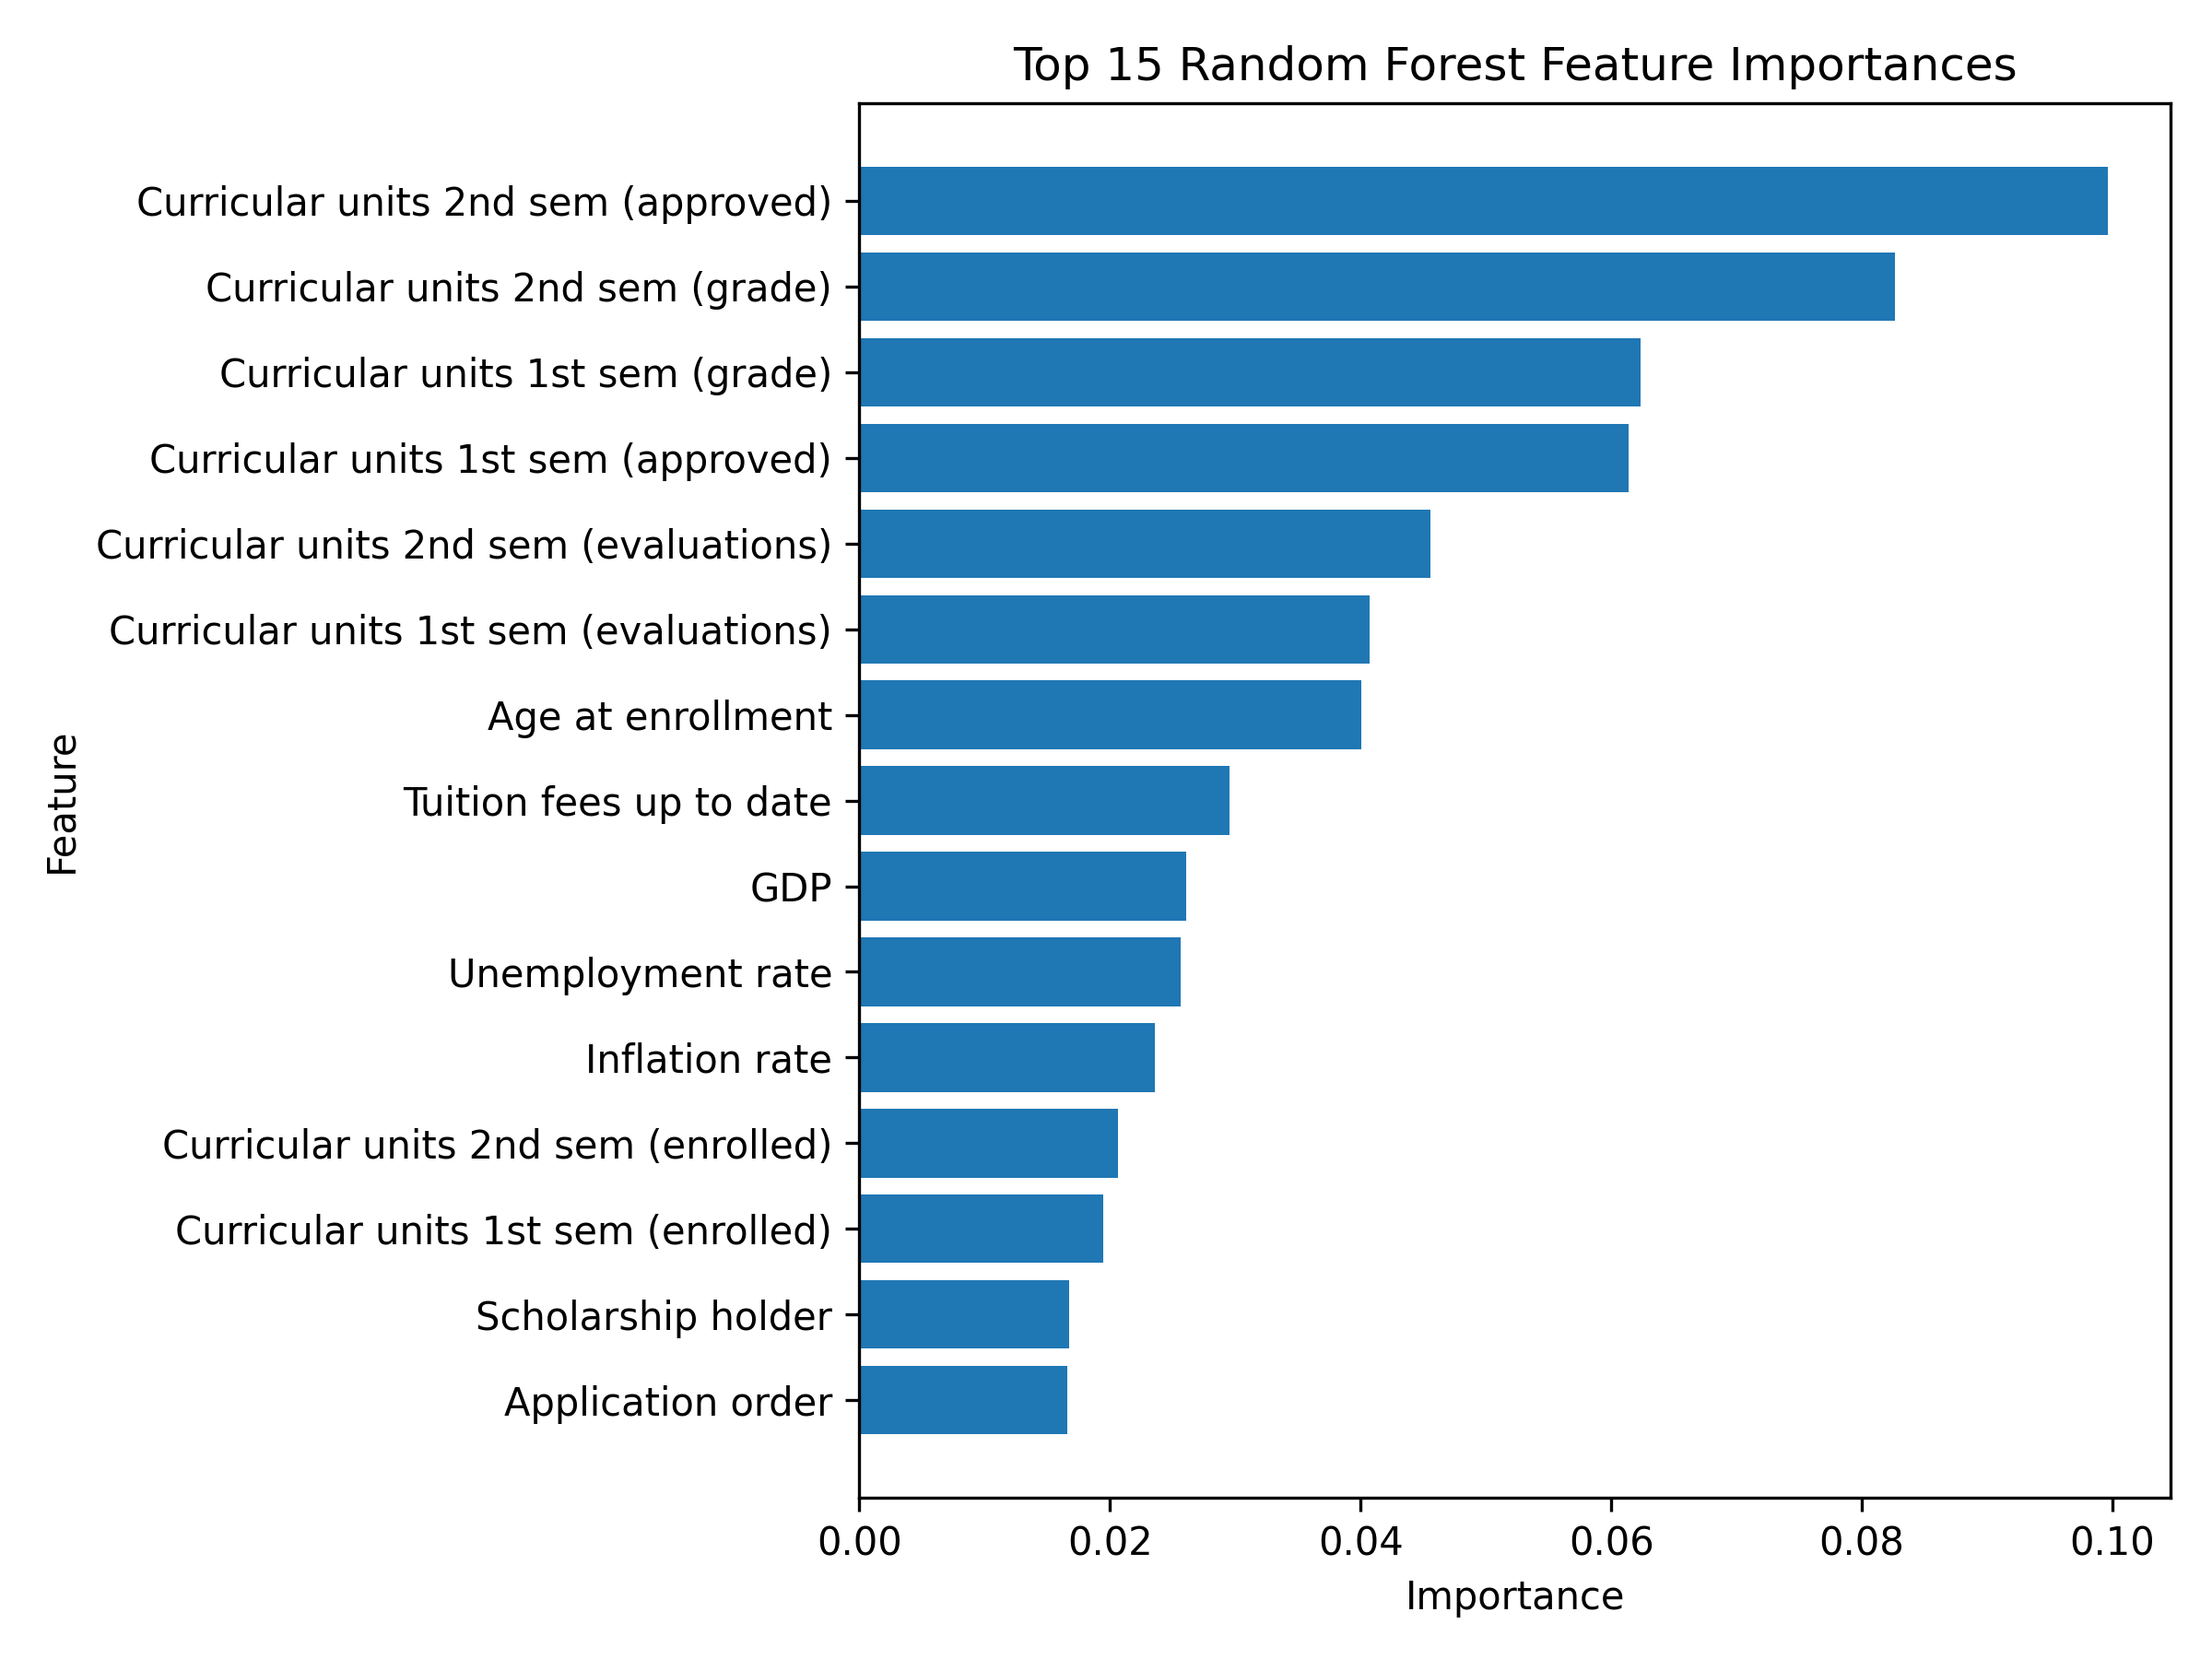
\includegraphics[width=0.85\linewidth]{figures/random_forest_feature_importance.png}
    \caption{Top 15 feature importances from the baseline Random Forest. Academic progress variables dominate the feature rankings.}
    \label{fig:feature_importance}
\end{figure}

\FloatBarrier

\section{Discussion}

The experiments show that standard supervised learning methods can predict student academic outcomes with reasonable accuracy from structured institutional data. The baseline Random Forest achieved the best accuracy and macro ROC-AUC, indicating strong overall discriminative ability. This result is consistent with the expectation that tree-based ensembles are effective for tabular data because they can capture nonlinear feature interactions without requiring heavy feature engineering.

However, the Logistic Regression model achieved the highest macro F1-score. This is important because the dataset is imbalanced and the \textit{Enrolled} class is more difficult to predict than the other two classes. The confusion matrices show that Random Forest is very strong at recognizing \textit{Graduate} students, but Logistic Regression provides a more balanced class-level trade-off. Therefore, the best model depends on the institutional goal. If the goal is overall ranking and separation, Random Forest is preferable. If the goal is balanced treatment of all classes, Logistic Regression may be more appropriate.

The clustering results provide a useful interpretability layer. K-Means identified a high-risk cluster in which 82.0\% of students were labeled as \textit{Dropout}. This cluster had extremely low academic progress, especially in curricular units approved and second-semester grade. In contrast, the other two clusters were majority-graduate groups with stronger academic performance. These results suggest that unsupervised segmentation can help institutions summarize student populations into interpretable groups.

At the same time, adding cluster labels to the supervised models did not consistently improve predictive performance. This does not mean clustering was useless. Instead, it suggests that the original feature space already contained the information captured by K-Means. The cluster labels compressed that information into a small number of group indicators, which helped interpretation but did not add much new predictive signal. This distinction is important: in applied machine learning, a technique may improve understanding without improving accuracy.

\section{Limitations}

This project has several limitations. First, the dataset comes from a specific higher-education context, so the trained models may not generalize directly to other universities, countries, or academic systems. Institutional policies, grading practices, economic conditions, and student support systems vary widely across contexts.

Second, the dataset includes first- and second-semester academic performance variables. These features are highly predictive, but they may not be available early enough for some intervention settings. If an institution wants to predict dropout risk before a student completes the first semester, a different feature set would be required. A useful future experiment would compare models trained with only pre-enrollment variables against models trained with semester performance data.

Third, the project uses K-Means clustering, which assumes roughly spherical clusters in the transformed feature space and is sensitive to preprocessing choices. Other clustering methods, such as Gaussian mixture models, hierarchical clustering, or density-based clustering, may reveal different student profiles.

Fourth, feature importance from Random Forest provides a useful but limited interpretation of model behavior. Future work could use SHAP values or partial dependence plots to provide more detailed explanations of how individual features affect predictions.

Finally, the project evaluates predictive performance on a single train-test split. Cross-validation could provide a more stable estimate of model performance and reduce dependence on one random split.

\section{Conclusion}

This project developed a hybrid clustering and classification framework for predicting student dropout and academic success. Using a higher-education retention dataset, I compared baseline supervised models with cluster-augmented models that incorporated K-Means student segments. The baseline Random Forest achieved the strongest overall performance, with 0.7605 accuracy and 0.8902 macro ROC-AUC. Logistic Regression achieved the highest macro F1-score, reflecting a more balanced treatment of the three outcome classes.

The cluster analysis revealed interpretable student profiles, including a high-risk cluster with 82.0\% dropout. However, adding cluster labels as model features did not consistently improve predictive performance. The main conclusion is that clustering is valuable for interpretation and student segmentation, while supervised models, especially Random Forest, are more effective for direct prediction. Future work should evaluate earlier intervention settings, compare additional clustering methods, and use more advanced explainability tools to support transparent decision-making in educational analytics.


\section*{AI Usage Disclosure}
The large language model GPT 5.5, was used to assist with project planning, code generation, debugging, experiment design, interpretation of results, and manuscript drafting. All experiments, figures, and reported metrics were created from the dataset and code included in the accompanying GitHub repository.

Code repository: \href{https://github.com/zackadam0/CS439-student-retention-project}{github.com/zackadam0/CS439-student-retention-project}.

\bibliographystyle{plainnat}
\bibliography{references}
\end{document}